\documentclass[a4paper, 14pt]{extarticle}

\usepackage{../../latexDependencies/misc/preamble}

\geometry{a4paper}

\begin{document}

\newgeometry{left=25mm, right=25mm, top=20mm, bottom=20mm}

\graphicspath{ {images} } 

% Customize section, subsection, subsubsection and paragraph styles
\titleformat{\section}
  {\normalfont\large\bfseries}{\thesection}{1em}{}

\titleformat{\subsection}
  {\normalfont\normalsize\bfseries}{\thesubsection}{1em}{}

\titleformat{\subsubsection}
  {\normalfont\small\bfseries}{\thesubsubsection}{1em}{}

\titleformat{\paragraph}
  {\small\small\bfseries}{\theparagraph}{1em}{}

\setcounter{tocdepth}{5}
\setcounter{secnumdepth}{5}

\pagenumbering{roman}

\tableofcontents\newpage

\pagenumbering{arabic}
\setcounter{page}{1}

\setstretch{1}
\linespread{1.1}

\setlength{\parindent}{0pt}

\fontsize{12pt}{16pt}\selectfont

\definecolor{myblue}{HTML}{0A88C2}
\definecolor{myred}{HTML}{FF1B1C}
\definecolor{mygreen}{HTML}{386641}

\lstdefinestyle{mystyle}{
    basicstyle=\ttfamily\footnotesize,
    keywordstyle=\color{myblue},
    stringstyle=\color{myred},
    commentstyle=\color{green!50!black},
    showstringspaces=false,
    frame=leftline, 
    framesep=10pt, 
}

% Set the style for Python code
\lstset{style=mystyle, extendedchars=\true}

% --------------------------------------START--------------------------------------

\section*{Задание}\vspace{-20pt}\rule{\linewidth}{0.1mm}
\addcontentsline{toc}{section}{Задание}

\begin{enumerate}
    \item Описать исходные данные, привести примеры задач, в которых могут возникнуть подобные исходные данные, описать используемый метод решения задачи и обосновать его применение;
    \item Проанализировать исходные данные. Изобразить исходные данные графически при помощи библиотеки matplotlib, привести код для построения значений. Подобрать вид функции, наилучшим образом описывающие исходные данные, обосновать выбор именно этого вида функции;
    \item Решить задачу аналитически. Описать нахождение коэффициентов выбранной функции методом наименьших квадратов вручную, с построением промежуточных таблиц значений. Полученный результат изобразить графически при помощи библиотеки matplotlib, привести код для построения значений; (Аналитическое решение можно выполнить от руки, приложить в отчет отсканированные фото)
    \item Решить задачу на языке python с использованием библиотеки numpy, привести код, привести результат решения. Полученный результат изобразить графически при помощи библиотеки matplotlib, привести код для построения значений;
    \item Решить задачу на языке python с использованием библиотеки scipy и matplotlib. Полученный результат изобразить графически при помощи библиотеки matplotlib, привести код для построения значений;
    \item Сравнить решения, полученные вручную и с помощью решения на python, построить решения графически.  Оценить точность полученных решений.
    \item С помощью полученной модели предсказать значения y для значений x = 4,5; x = 5.
\end{enumerate}

\section*{Исходные данные}\vspace{-20pt}\rule{\linewidth}{0.1mm}
\addcontentsline{toc}{section}{Исходные данные}

\begin{table}[h!]
    \centering
    \begin{adjustbox}{max width=1\textwidth}
    \setlength{\tabcolsep}{20pt} % Increase the horizontal space between columns
    \begin{tabular}{l!{\vrule width 1pt}cccccc}
        \toprule
        x & 3 & 5 & 7 & 9 & 11 & 13 \\
        y & 3.5 & 4.4 & 5.7 & 6.1 & 6.5 & 7.3 \\
        \bottomrule
    \end{tabular}
    \end{adjustbox}
    \caption{Исходные данные}
    \label{tab:sample_table}
\end{table}

\section*{{Ход решения}}
\addcontentsline{toc}{section}{Ход решения}

\subsection*{{Часть 1}}\vspace{-20pt}\rule{\linewidth}{0.1mm}
\addcontentsline{toc}{subsection}{Часть 1}

\vspace{-10pt} Описать исходные данные, привести примеры задач, в которых могут возникнуть 
подобные исходные данные, описать используемый метод решения задачи и обосновать его 
применение;\\

Исходными данными являются некоторые результаты наблюдений, представленные в таблице 1. Данные 
равномерно распределены на небольшом промежутке по оси абсцисс и монотонно возрастают по оси ординат. 
Похожие данные можно много где увидеть. Например стоимость золота за небольшой временной период будет 
иметь похожий вид. В качестве другого примера можно привести статистику роста населения.\\

Используемый метод решения задачи – Метод наименьших квадратов (МНК).\\

\subsubsection*{{Описание работы МНК}}\vspace{-20pt}\rule{\linewidth}{0.1mm}
\addcontentsline{toc}{subsubsection}{Описание работы МНК}

\subsubsection*{{Обоснование применения МНК}}\vspace{-20pt}\rule{\linewidth}{0.1mm}
\addcontentsline{toc}{subsubsection}{Обоснование применения МНК}

Метод наименьших квадратов широко применяется в различных областях науки и практики, 
и используется для подбора зависимости, которые лучше всего соответствуют набору данных. \\

Применение метода наименьших квадратов обосновано для этой задачи, потому что метод 
обладает рядом преимуществ: \\

\begin{itemize}
    \item[--] Простота использования: МНК не требует сложных вычислений или предположений о распределении данных. 
    \item[--] Точность: МНК обеспечивает высокую точность предсказаний, так как он минимизирует сумму квадратов ошибок между наблюдаемыми и предсказанными значениями.
    \item[--] Универсальность: МНК может использоваться для решения широкого круга задач, таких как прогнозирование временных рядов, регрессионный анализ, аппроксимация функций и т.д.
    \item[--] Применимость: МНК применим к данным, которые имеют в том числе нелинейную зависимость между переменными. 
\end{itemize}

\subsubsection*{{Примеры задач}}\vspace{-20pt}\rule{\linewidth}{0.1mm}
\addcontentsline{toc}{subsubsection}{Примеры задач}

Примеры задач, в которых могут возникнуть подобные исходные данные и может применяться МНК: 

\begin{itemize}
    \item Прогноз погоды: Метеорологическая станция может собирать данные о температуре и влажности в течение определенного периода времени. Используя МНК, можно определить наилучшую линию, которая предсказывает температуру в зависимости от влажности.
    \item Анализ спроса на товары: Магазин может собирать данные об объемах продаж определенных товаров в зависимости от дня недели. Используя МНК, можно выявить закономерности и определить, в какие дни спрос на товары увеличивается или уменьшается.
    \item Прогнозирование продаж: Компания может собирать данные о продажах своих продуктов в разных регионах в течение нескольких месяцев. МНК может быть использован для определения наилучшей линии, предсказывающей продажи продуктов в зависимости от региона.
    \item Финансовый анализ: Аналитик может собирать исторические данные о ценах акций и объемах торгов. МНК можно использовать для определения оптимальной линии, которая предскажет будущие цены акций на основе исторических данных.
    \item Геофизика: Геофизики могут использовать МНК для анализа гравитационных и магнитных полей и определения наличия залежей полезных ископаемых под землей.
\end{itemize}

\newpage

\subsection*{{Часть 2}}\vspace{-20pt}\rule{\linewidth}{0.1mm}
\addcontentsline{toc}{subsection}{Часть 2}

Проанализировать исходные данные. Изобразить исходные данные графически при помощи 
библиотеки matplotlib, привести код для построения значений. Подобрать вид функции, 
наилучшим образом описывающие исходные данные, обосновать выбор именно этого вида функции; \\

\subsubsection*{{Построение исходных графиков}}\vspace{-20pt}\rule{\linewidth}{0.1mm}
\addcontentsline{toc}{subsubsection}{Построение исходных графиков}

Изобразим исходные данные графически при помощи библиотеки matplotlib. \\
Для начала подключим все необходимые библиотеки:

\begin{center}
    \begin{lstlisting}[language=Python]
import matplotlib.pyplot as plt
import matplotlib.font_manager as fm
from fontTools.ttLib import TTFont

from dataclasses import dataclass
from typing import Callable

from IPython.display import Math, Latex, display

import sympy

import scipy as sp
import numpy as np

font_path = '../../extra/Cinzel-VariableFont_wght.ttf'

cinzel_font = fm.FontProperties(fname=font_path)
fm.fontManager.addfont(font_path)
    \end{lstlisting}
\end{center}

Заведем несколько констант, которые в дальнейшем будем использовать при построении графиков:

\begin{center}
    \begin{lstlisting}[language=Python]
SAVE_PLOTS = True
RED = '#6F1D1B'
RICH_BLACK = '#011627'
    \end{lstlisting}
\end{center}

А так же запишем исходные данные:

\begin{center}
    \begin{lstlisting}[language=Python]
x_values_ = [3, 5, 7, 9, 11, 13]
y_values_ = [3.5, 4.4, 5.7, 6.1, 6.5, 7.3]
n_ = len(x_values_)
    \end{lstlisting}
\end{center}

Заведем вспомогательную функцию для настройки внешнего вида всех дальнейших графиков:

\begin{center}
    \begin{lstlisting}[language=Python]
def decorate_plot(ax, x_ticks, xname, yname, loc):
    SIZE_TICKS = 12

    # Eliminate upper and right axes
    ax.spines['right'].set_color('none')
    ax.spines['top'].set_color('none')

    # Show ticks in the left and lower axes only
    ax.xaxis.set_ticks_position('bottom')
    ax.yaxis.set_ticks_position('left')

    # x axis name
    ax.set_xlabel(xname, fontsize=15)
    ax.xaxis.set_label_coords(0.98, 0.05)

    # y axis name
    ax.set_ylabel(yname, rotation=0, fontsize=15)
    ax.yaxis.set_label_coords(0.025, 0.95)

    ax.set_xticks(x_ticks)

    # Adjust the font size of the tick labels
    ax.tick_params(axis='both', which='major', labelsize=SIZE_TICKS)

    if loc:
        plt.legend(fontsize=10, loc=loc)

    # Update font settings
    plt.rcParams.update({
        "font.family": cinzel_font.get_name(), 
        "font.size": 16
    })

    # Adjust layout
    plt.tight_layout()
    \end{lstlisting}
\end{center}

Наконец запишем функцию для отображения самого графика:

\begin{center}
    \begin{lstlisting}[language=Python]
def buildClassicBar(filename, plotname, x_values, y_values, type):
    _, ax = plt.subplots(figsize=(10, 6))

    match type:
        case 'scatter':
            ax.scatter(x_values, 
                       y_values, 
                       color=RED,
                       s=50)
        case 'plot':
            ax.plot(x_values, 
                    y_values, 
                    color=RED)
        case 'stem':
            ax.stem(x_values, 
                    y_values, 
                    color=RED)
        case 'stackplot':
            ax.stackplot(x_values, 
                         y_values, 
                         color=RED)

    plt.grid(linestyle='-', linewidth=0.25)

    ax.set_title(plotname)
    decorate_plot(ax, np.arange(x_values[0], x_values[-1]+1, 1), 'x', 'y', '')
    
    if SAVE_PLOTS:
        plt.savefig(f'images/{filename}.png', dpi=300, transparent=True)

    plt.show()
    \end{lstlisting}
\end{center}

Вызовем ее:

\begin{center}
    \begin{lstlisting}[language=Python]
buildClassicBar('initial_scatter_plot', 
                'Scatter Plot', 
                x_values_, 
                y_values_, 
                'scatter')
    \end{lstlisting}
\end{center}

Получим следующий график:

\begin{center}
    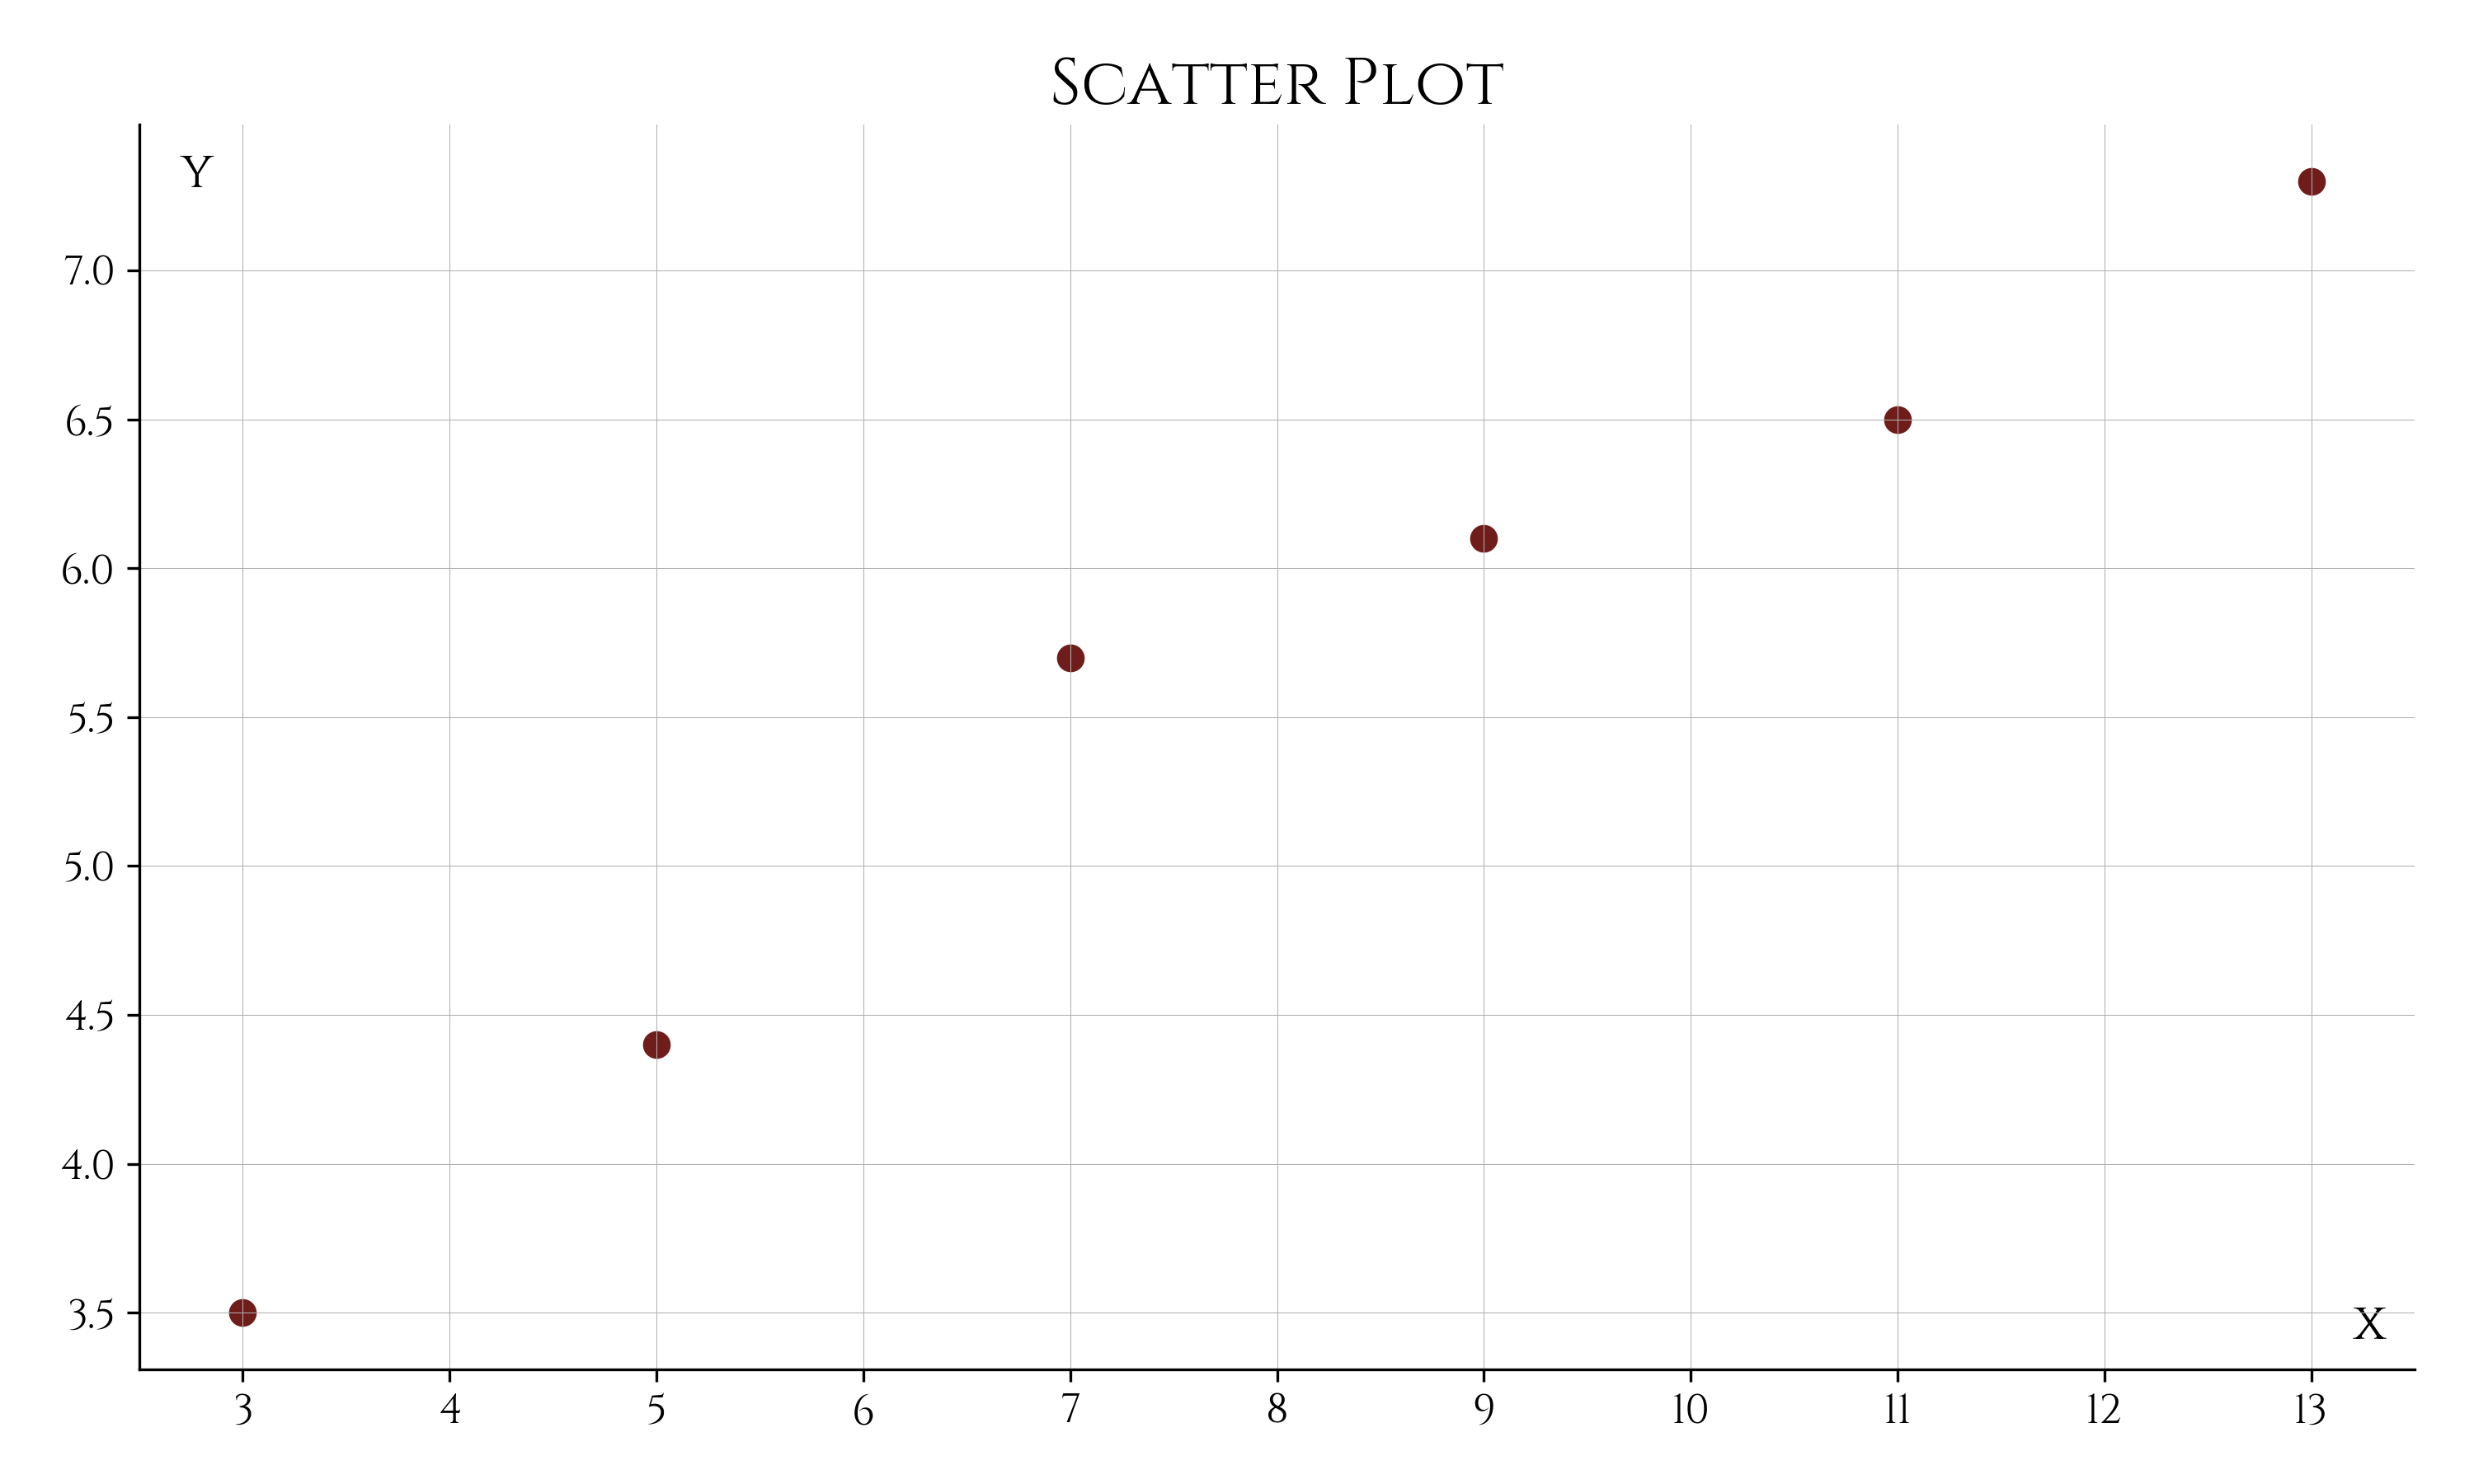
\includegraphics[width=1\textwidth, height=0.5\textheight, keepaspectratio]{initial_scatter_plot} \\
\end{center}

Также изобразим исходные данные в виде ломанной линии:

\begin{center}
    \begin{lstlisting}[language=Python]
buildClassicBar('initial_regular_plot', 
                'Regular Plot', 
                x_values_, 
                y_values_, 
                'plot')
    \end{lstlisting}
\end{center}

\begin{center}
    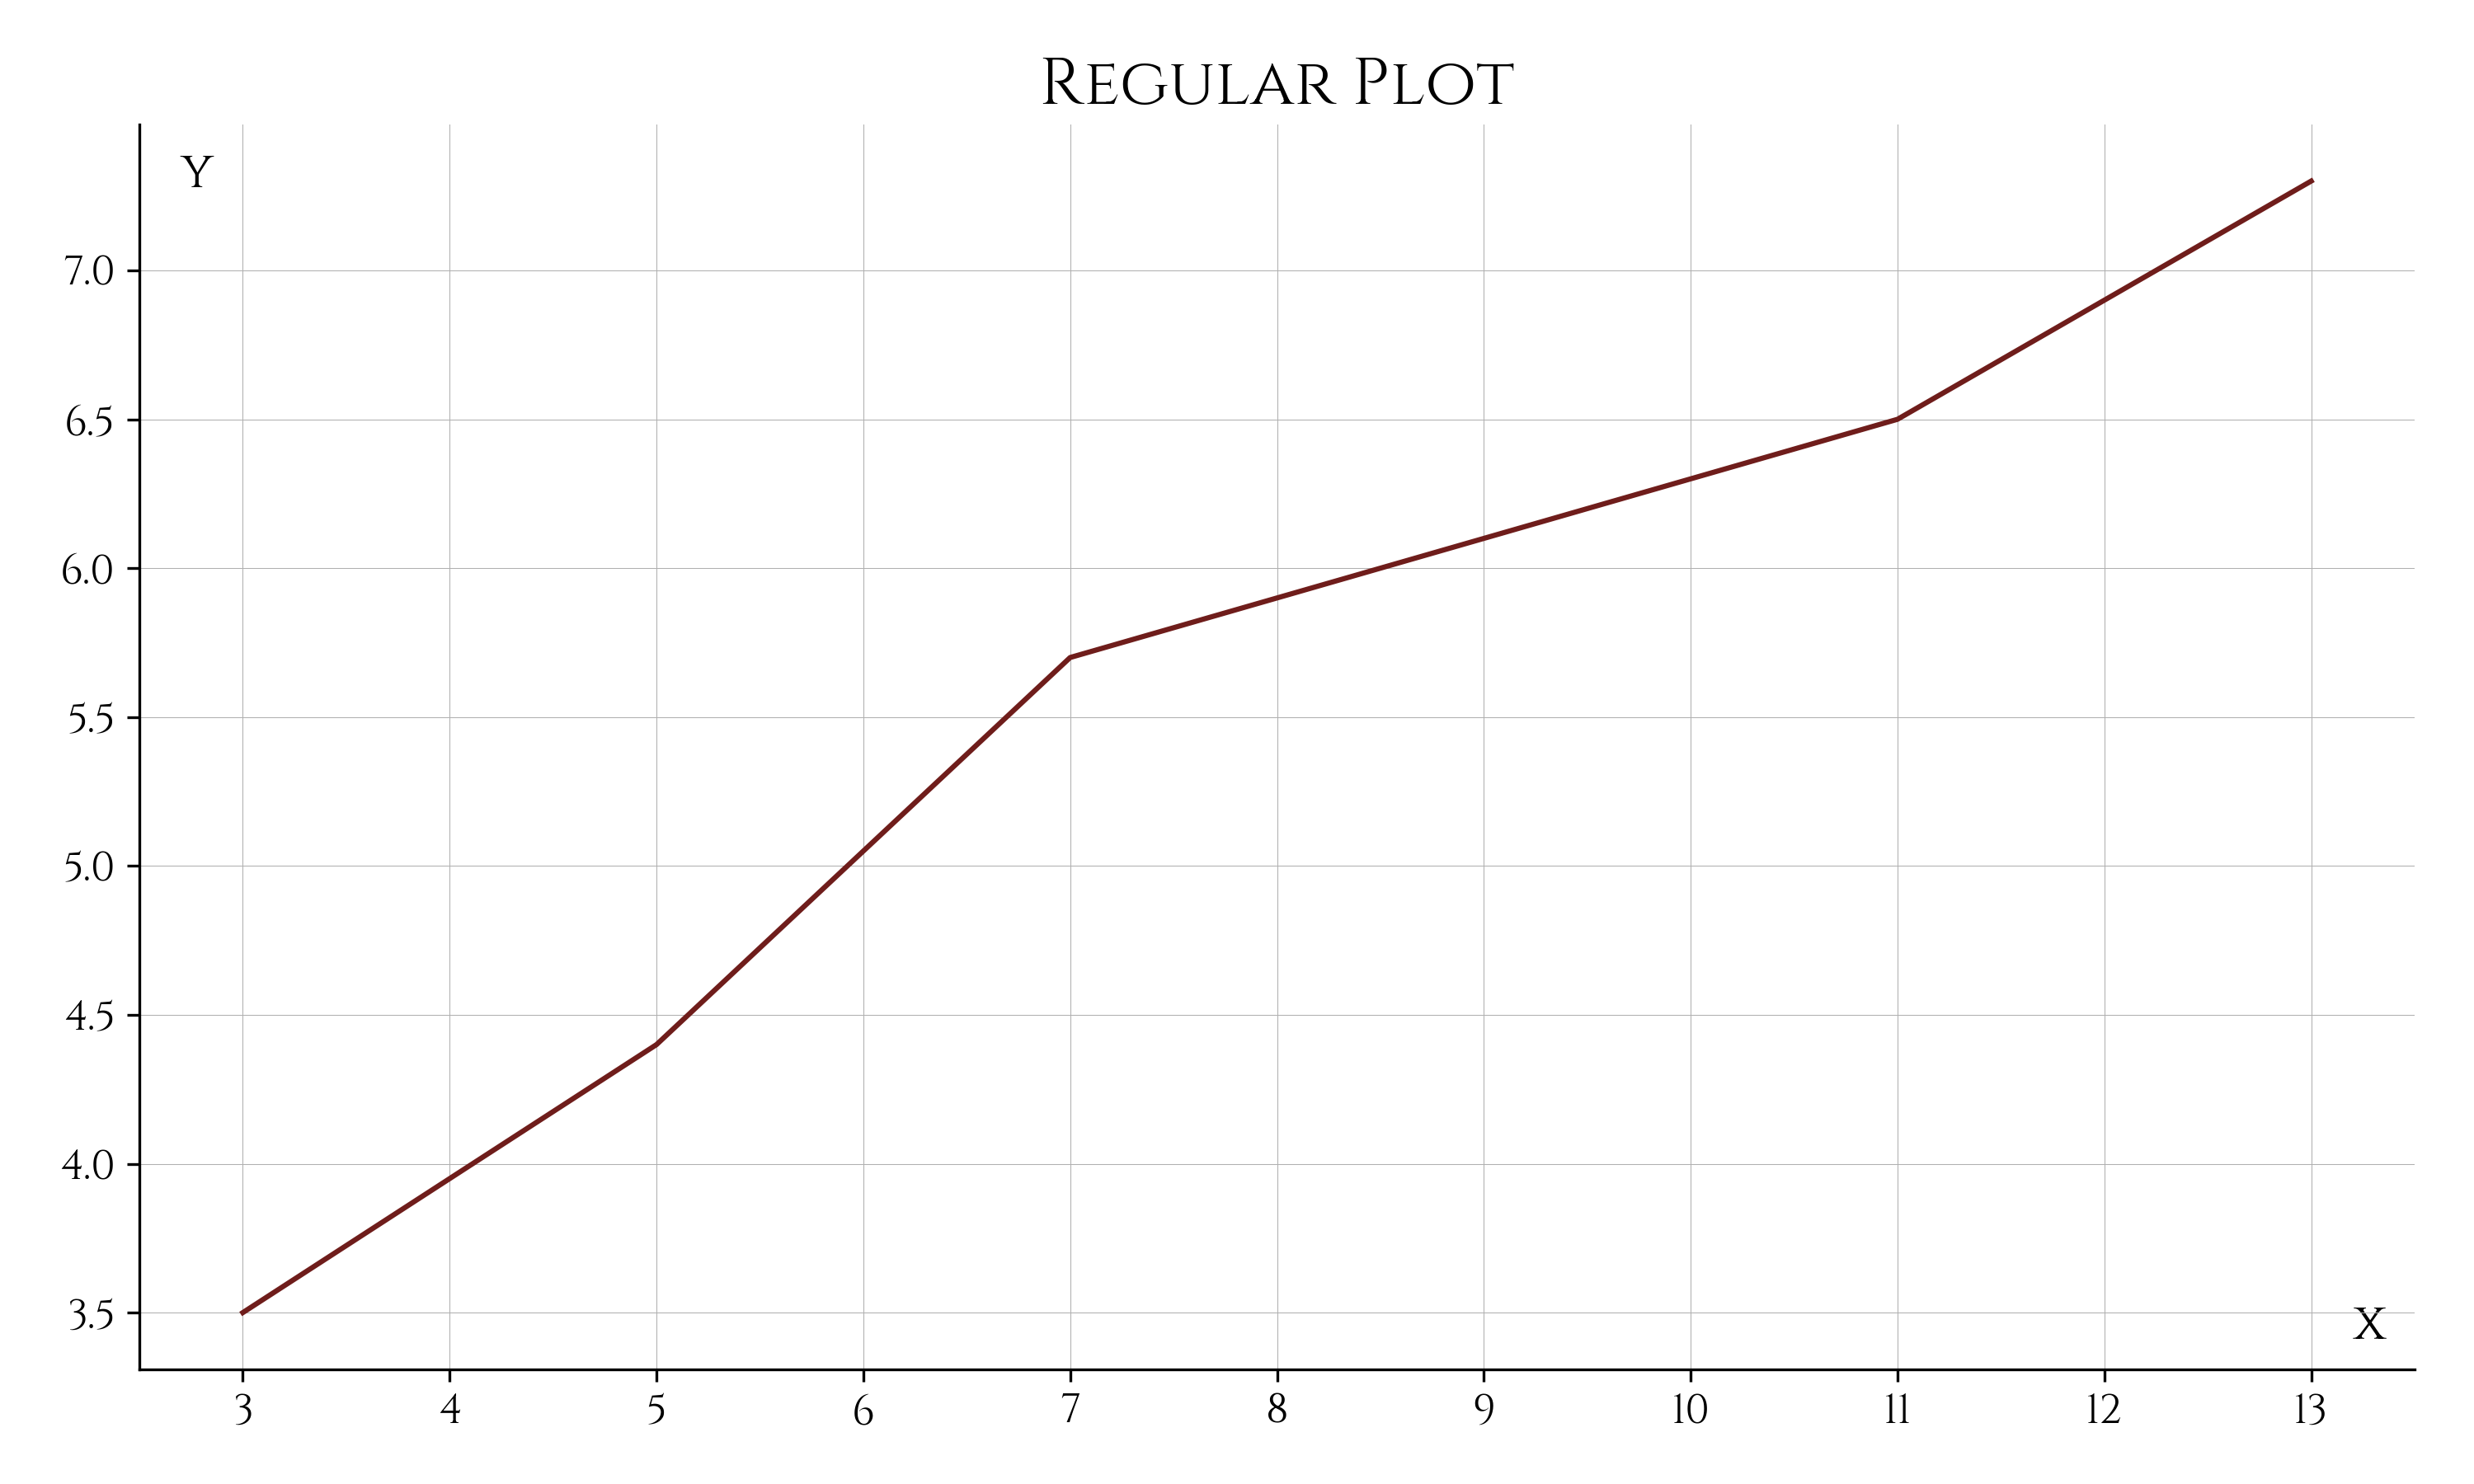
\includegraphics[width=1\textwidth, height=0.5\textheight, keepaspectratio]{initial_regular_plot} \\
\end{center}

\subsubsection*{{Подбор вида функции}}\vspace{-20pt}\rule{\linewidth}{0.1mm}
\addcontentsline{toc}{subsubsection}{Подбор вида функции}

Исходя из вида данных можно выдвинуть несколько предположений о виде функции. Наблюдая за 
интерпретацией данных на графике \high{Scatter Plot} можно сделать предположение, что данные 
имеют линейную зависимость. Однако если посмотреть на \high{Regular Plor}, то можно 
заметить, что данные имеют изгиб, который можно смоделировать кубической функцией. Далее 
мы рассмотрим оба эти случая.\\

В качестве доказательства первой гипотезы (о линейности данных), вручную подберем наиболее 
подходящую функцию:

\begin{equation*}
    y = \cfrac{1}{2.63} \cdot x - \cfrac{3}{2.63} + 3.7
\end{equation*}

Построим ее:

\newpage\vfill\null\null

\begin{center}
    \begin{lstlisting}[language=Python]
def buildBar(filename, plotName, plotTitle, x_values, 
                                            y_values, 
                                            new_x_values, 
                                            new_y_values):
    _, ax = plt.subplots(figsize=(10, 6))

    # initial scatter data
    ax.scatter(x_values, 
               y_values, 
               color=RED,
               label='Initial data',
               s=50)

    # approximation
    ax.plot(new_x_values, new_y_values, color=RICH_BLACK, label=plotName)

    plt.grid(linestyle='-', linewidth=0.25)

    ax.set_title(plotTitle)
    decorate_plot(ax, np.arange(new_x_values[0], 
                                new_x_values[-1]+1, 1), 'x', 'y', loc=(0.005, 
                                                                       0.825))
    
    if SAVE_PLOTS:
        plt.savefig(f'images/{filename}.png', dpi=300, transparent=True)

    plt.show()

new_x_values = np.linspace(0, x_values_[-1] + 3, 100)
a_hand = 2.63
b_hand = -3.7
hand_func = lambda x : 1/a_hand * x - 3/a_hand - b_hand
new_y_values = hand_func(new_x_values)

y_values_hand_approximation = new_y_values

buildBar('Plot_Hand_Approximation', 
         'Approximation', 
         'Hand Approximation', 
         x_values_, 
         y_values_, 
         new_x_values, 
         new_y_values)
    \end{lstlisting}
\end{center}

\vfill\newpage

\begin{center}
    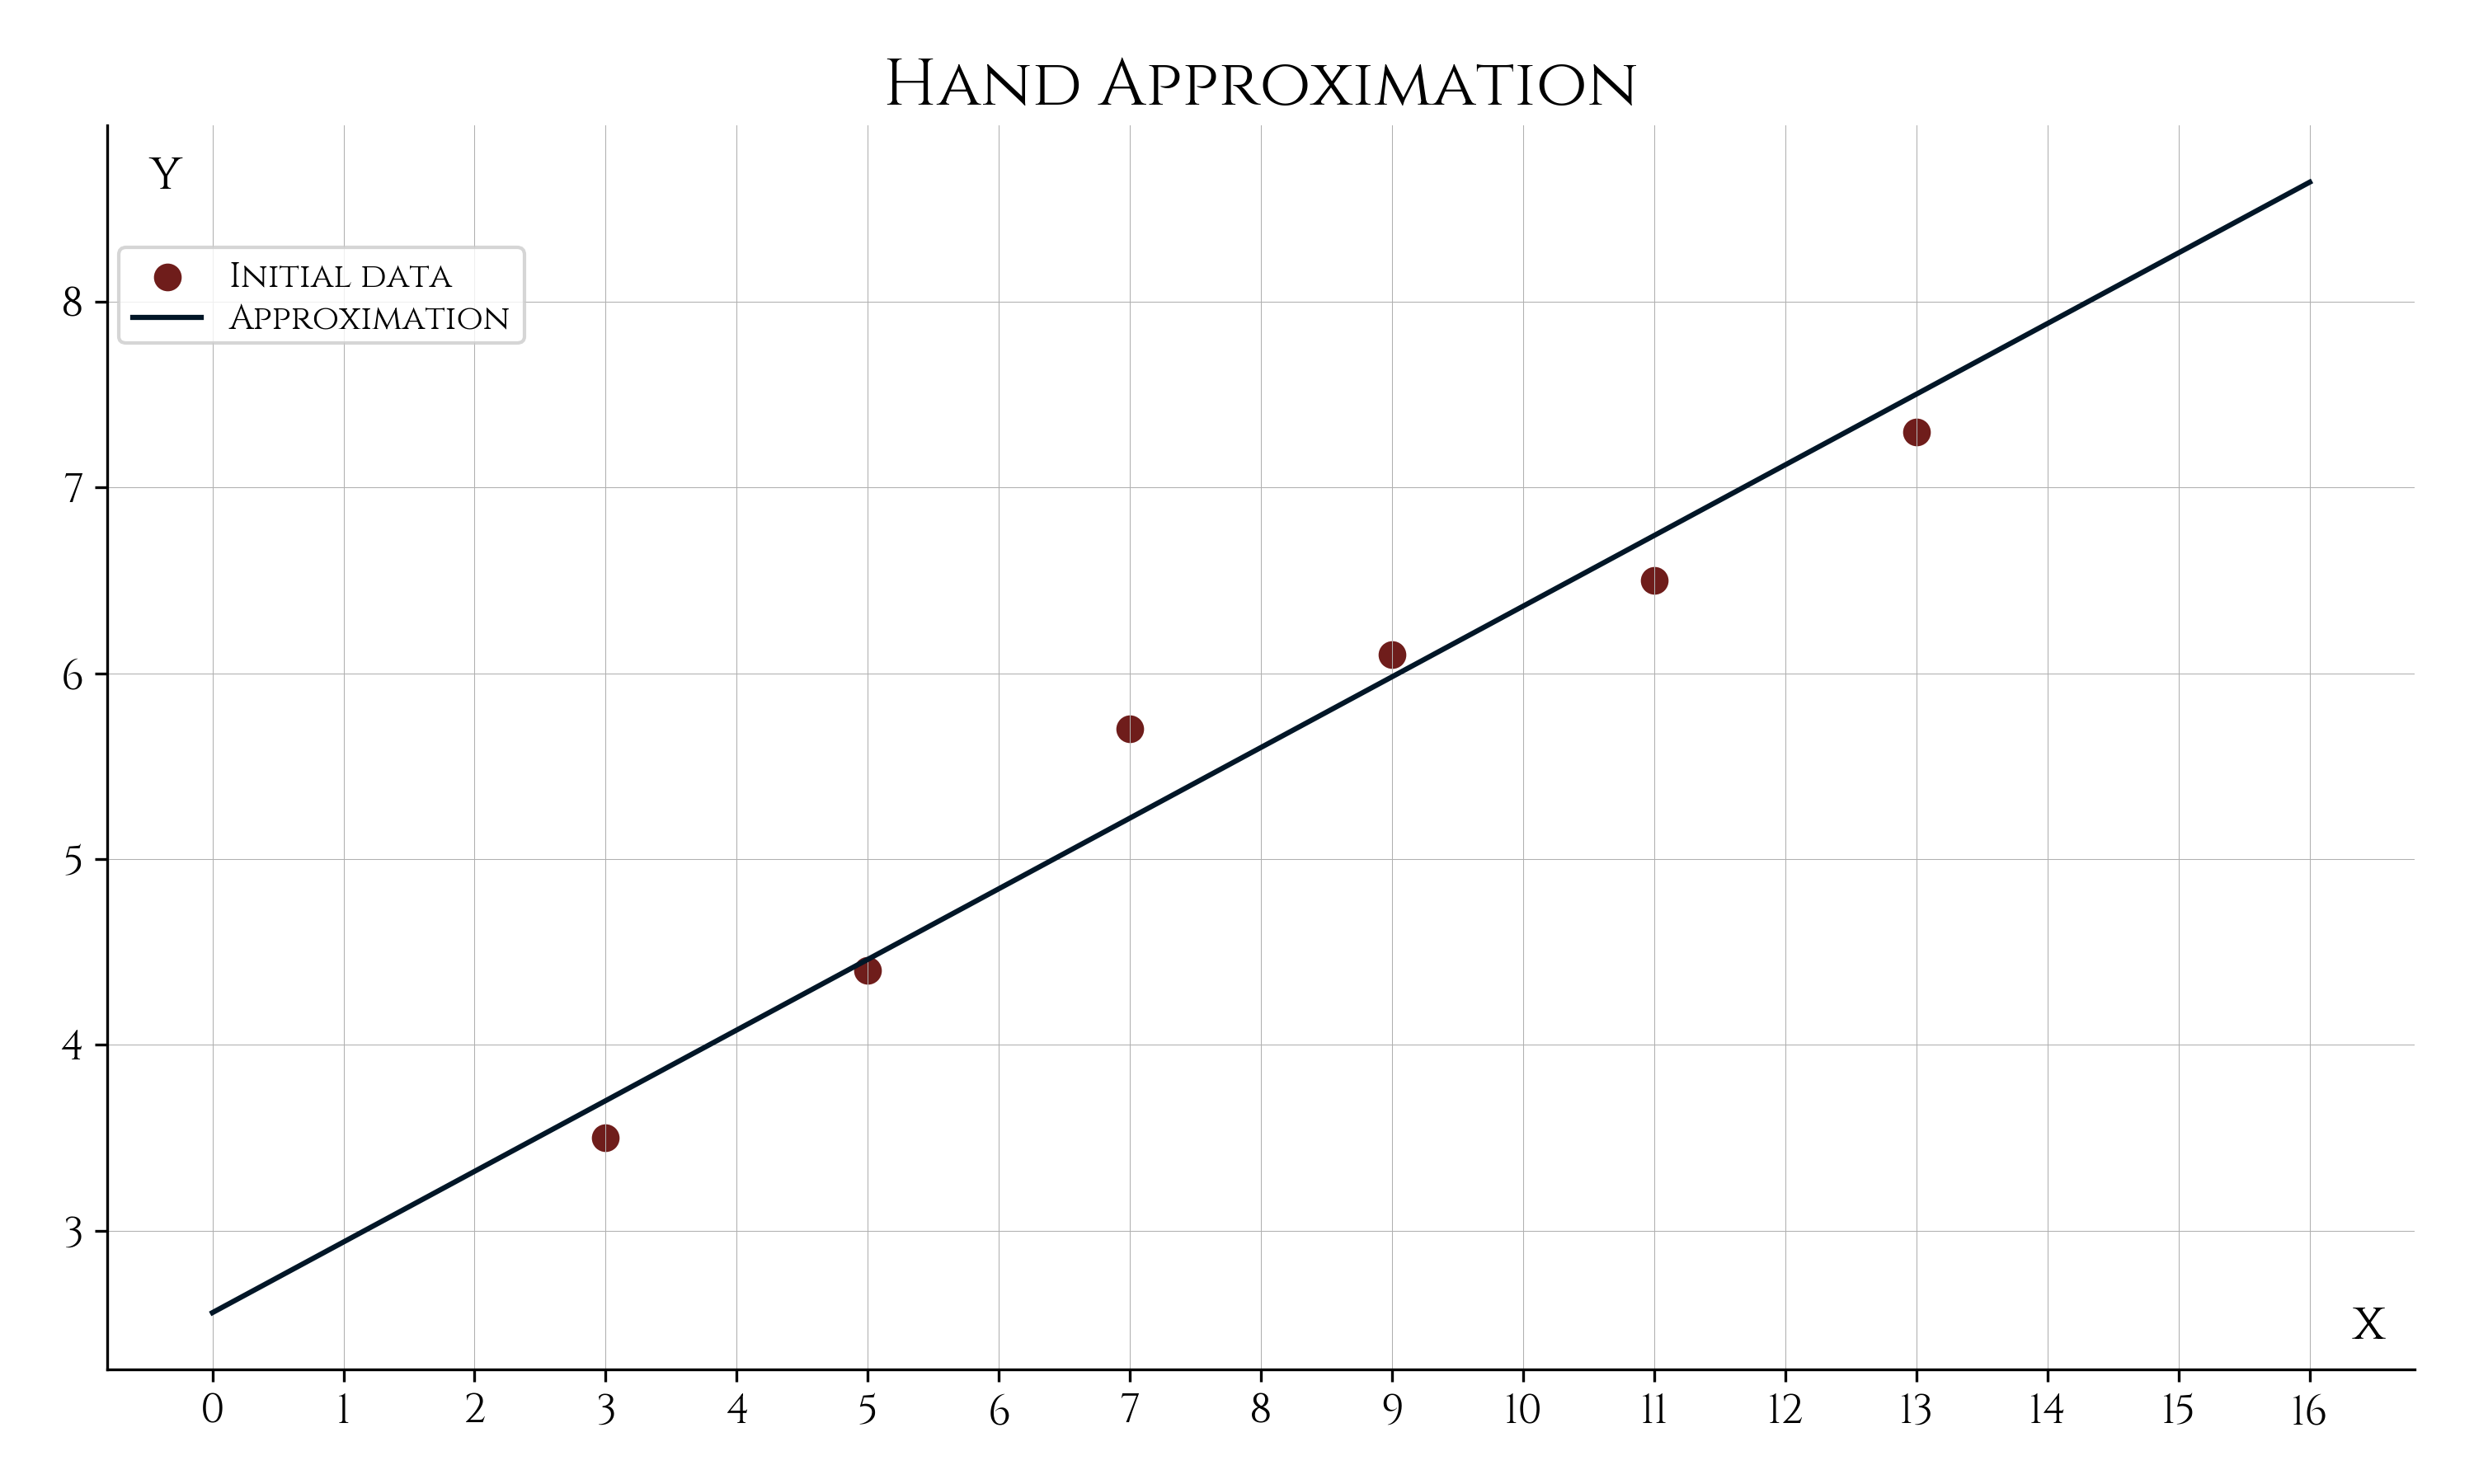
\includegraphics[width=1\textwidth, height=0.5\textheight, keepaspectratio]{Plot_Hand_Approximation} \\
\end{center}

\subsection*{{Часть 3}}\vspace{-20pt}\rule{\linewidth}{0.1mm}
\addcontentsline{toc}{subsection}{Часть 3}

Решить задачу аналитически. Описать нахождение коэффициентов выбранной функции методом 
наименьших квадратов вручную, с построением промежуточных таблиц значений. Полученный 
результат изобразить графически при помощи библиотеки matplotlib, привести код для построения 
значений; (Аналитическое решение можно выполнить от руки, приложить в отчет отсканированные фото)

\subsubsection*{{Линейная регрессия}}\vspace{-20pt}\rule{\linewidth}{0.1mm}
\addcontentsline{toc}{subsubsection}{Линейная регрессия}

Аналитически выразим формулы для коэффициентов парной линейной регрессии методом МНК.

\vfill

\begin{equation*}
    \scalebox{1.5}{
        $\downarrow$
    }
\end{equation*}

\vfill\newpage

\begin{center}
    \fbox{\includegraphics[width=1\textwidth, height=1\textheight, keepaspectratio]{Analyitcal_Linear_Regression_1}} \\
\end{center}

\begin{center}
    \fbox{\includegraphics[width=1\textwidth, height=1\textheight, keepaspectratio]{Analyitcal_Linear_Regression_2}} \\
\end{center}

\begin{center}
    \fbox{\includegraphics[width=1\textwidth, height=1\textheight, keepaspectratio]{Analyitcal_Linear_Regression_3}} \\
\end{center}

\begin{center}
    \fbox{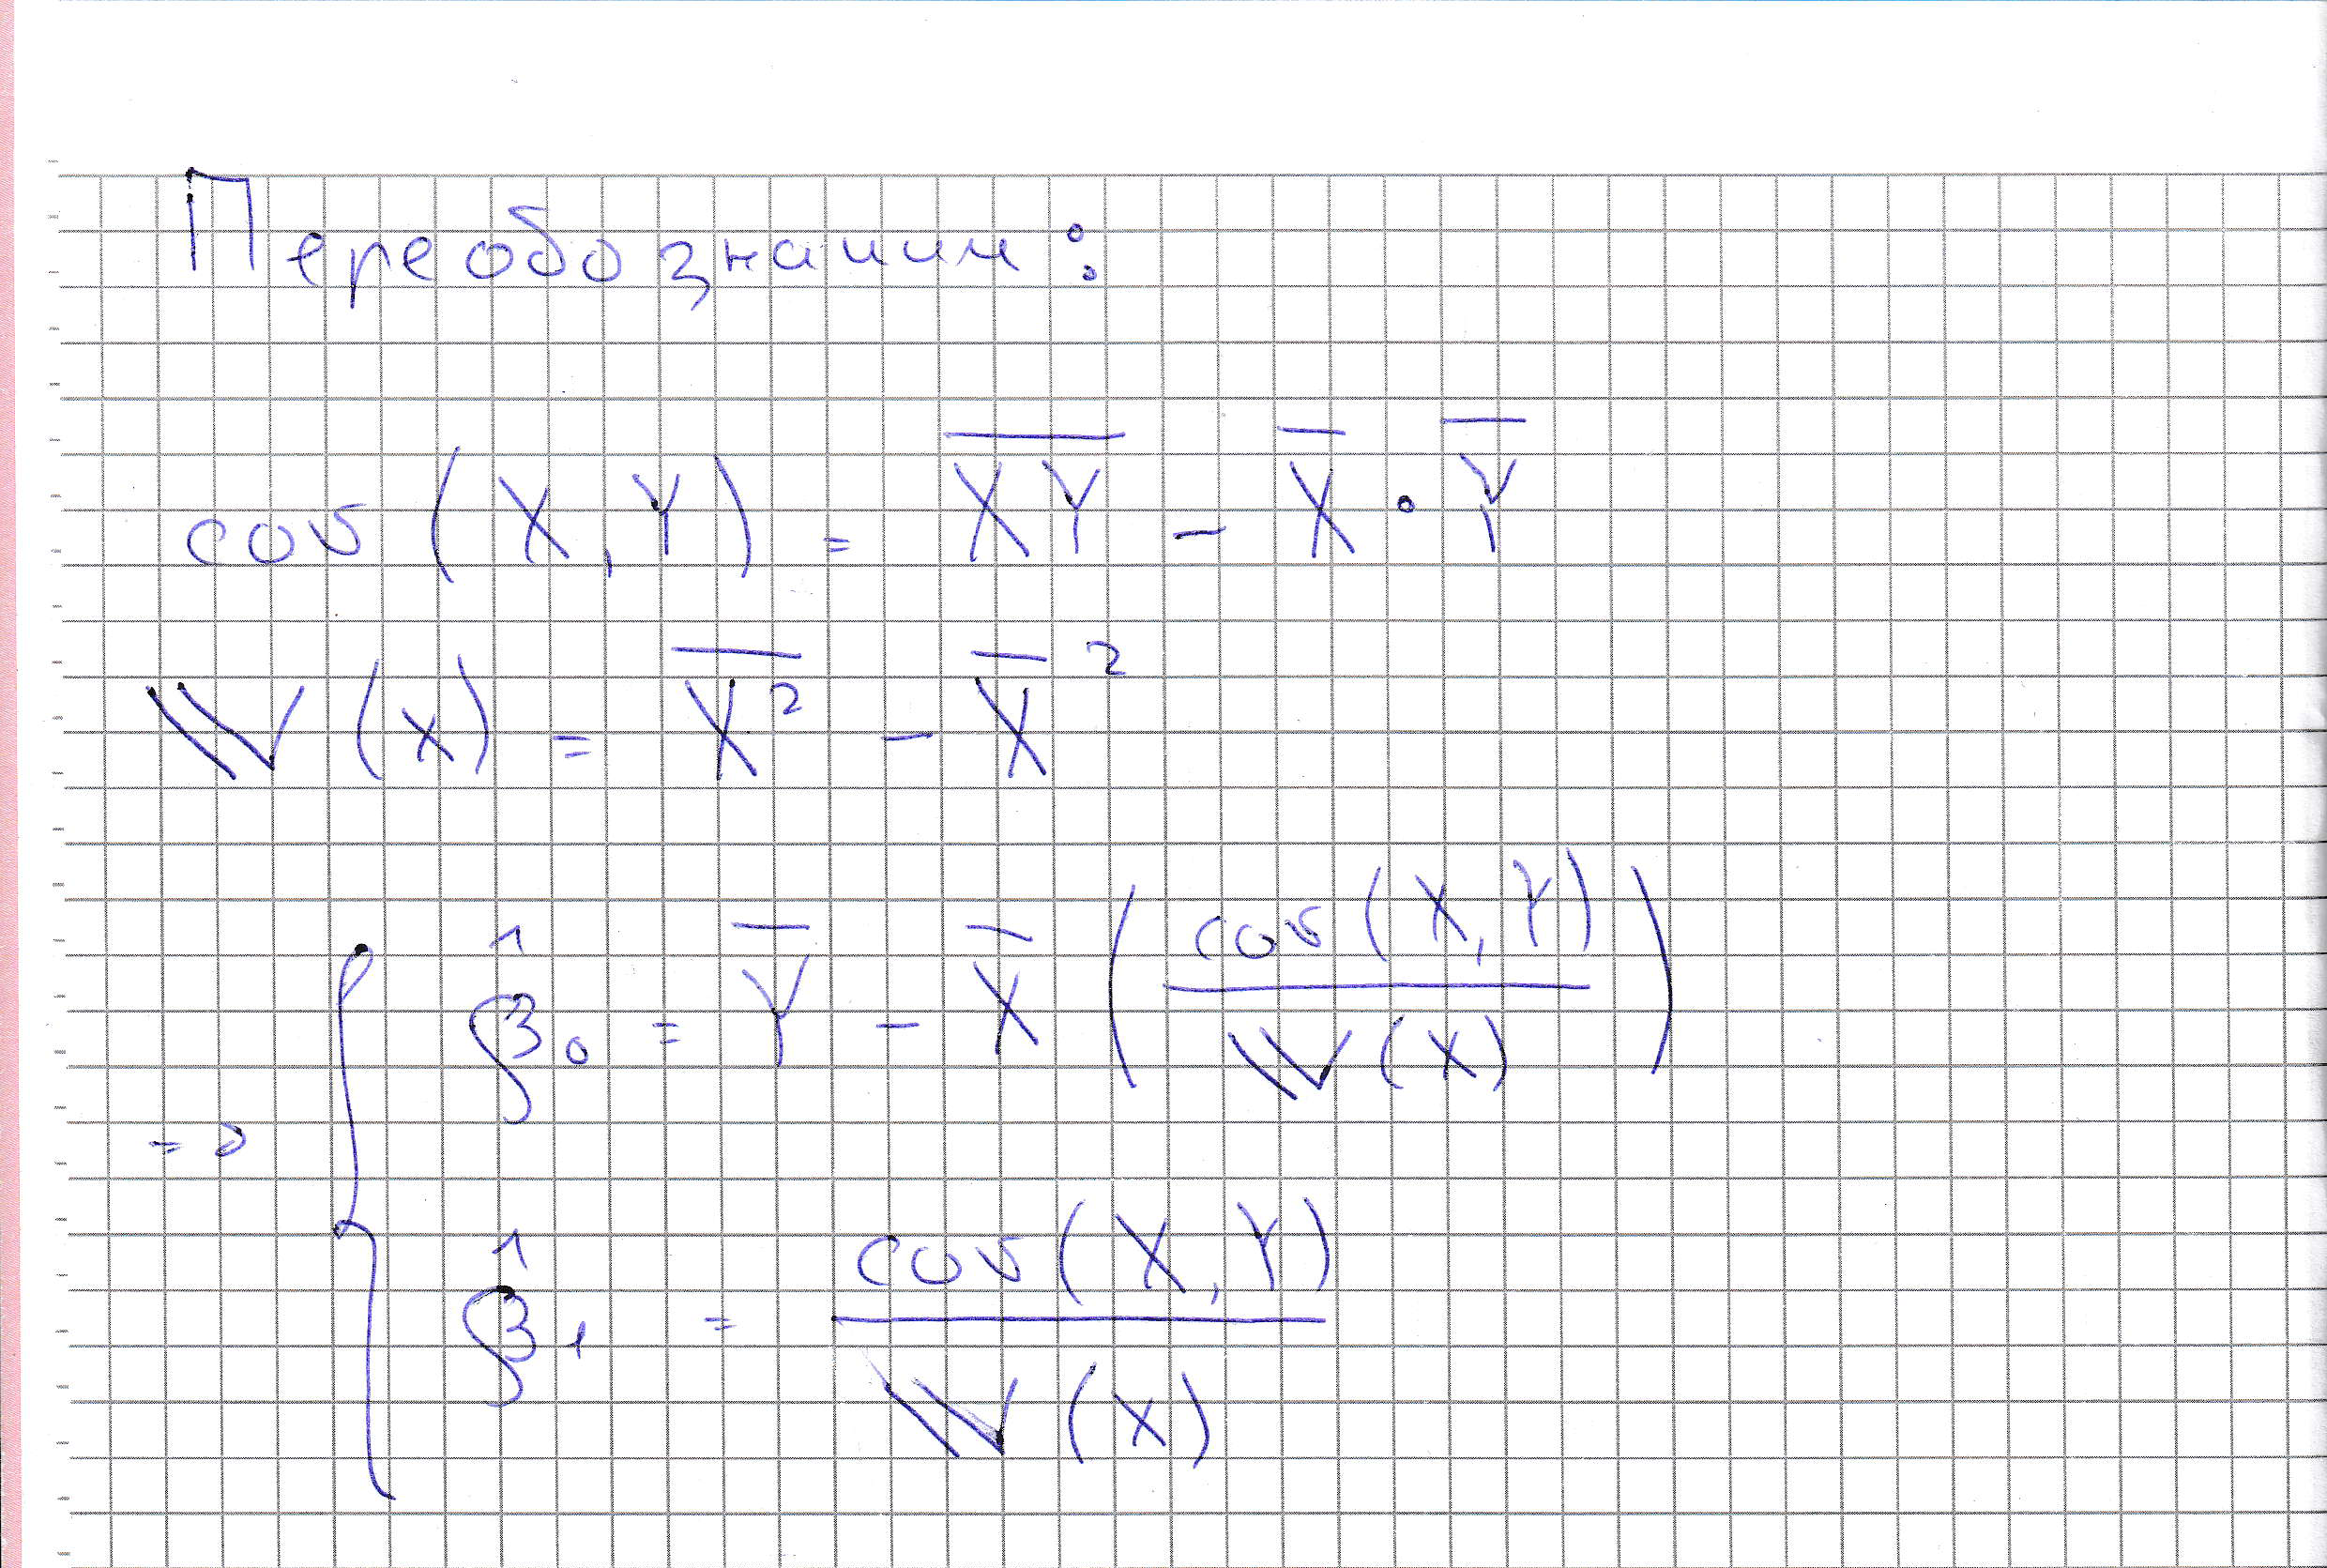
\includegraphics[width=1\textwidth, height=1\textheight, keepaspectratio]{Analyitcal_Linear_Regression_4}} \\
\end{center}

Теперь посчитаем найденные коэффициенты:

\begin{center}
    \begin{lstlisting}[language=Python]
overlineX = 1/n_ * sum(x_values_)
overlineY = 1/n_ * sum(y_values_)

overlineX2 = 1/n_ * sum([x**2 for x in x_values_])

overlineXY = 1/n_ * sum([x * y for x, y in zip(x_values_, y_values_)])

cov = overlineXY - overlineX * overlineY
Var = overlineX2 - overlineX**2

beta_0 = overlineY - overlineX * (cov/Var)
beta_1 = cov/Var

linear_analytical_beta = [beta_0, beta_1]

print(linear_analytical_beta)

linear_analytical_func = lambda x: linear_analytical_beta[0] + \
                                   linear_analytical_beta[1] * x
    \end{lstlisting}
\end{center}

Получим:

\begin{equation*}
    \beta_0 \approx 2.646 \qquad \beta_1 \approx 0.3671
\end{equation*}

Построим график полученной модели:

\begin{center}
    \begin{lstlisting}[language=Python]
new_x_values = np.linspace(0, x_values_[-1] + 3, 100)
new_y_values = linear_analytical_func(new_x_values)

y_values_linear_analytical = new_y_values

buildBar('Linear_Regression_Analytical', 
         '$\\hat{y}$', 
         'Linear Regression (using OLS)', 
         x_values_, 
         y_values_, 
         new_x_values, 
         new_y_values)
    \end{lstlisting}
\end{center}

Получим:

\begin{center}
    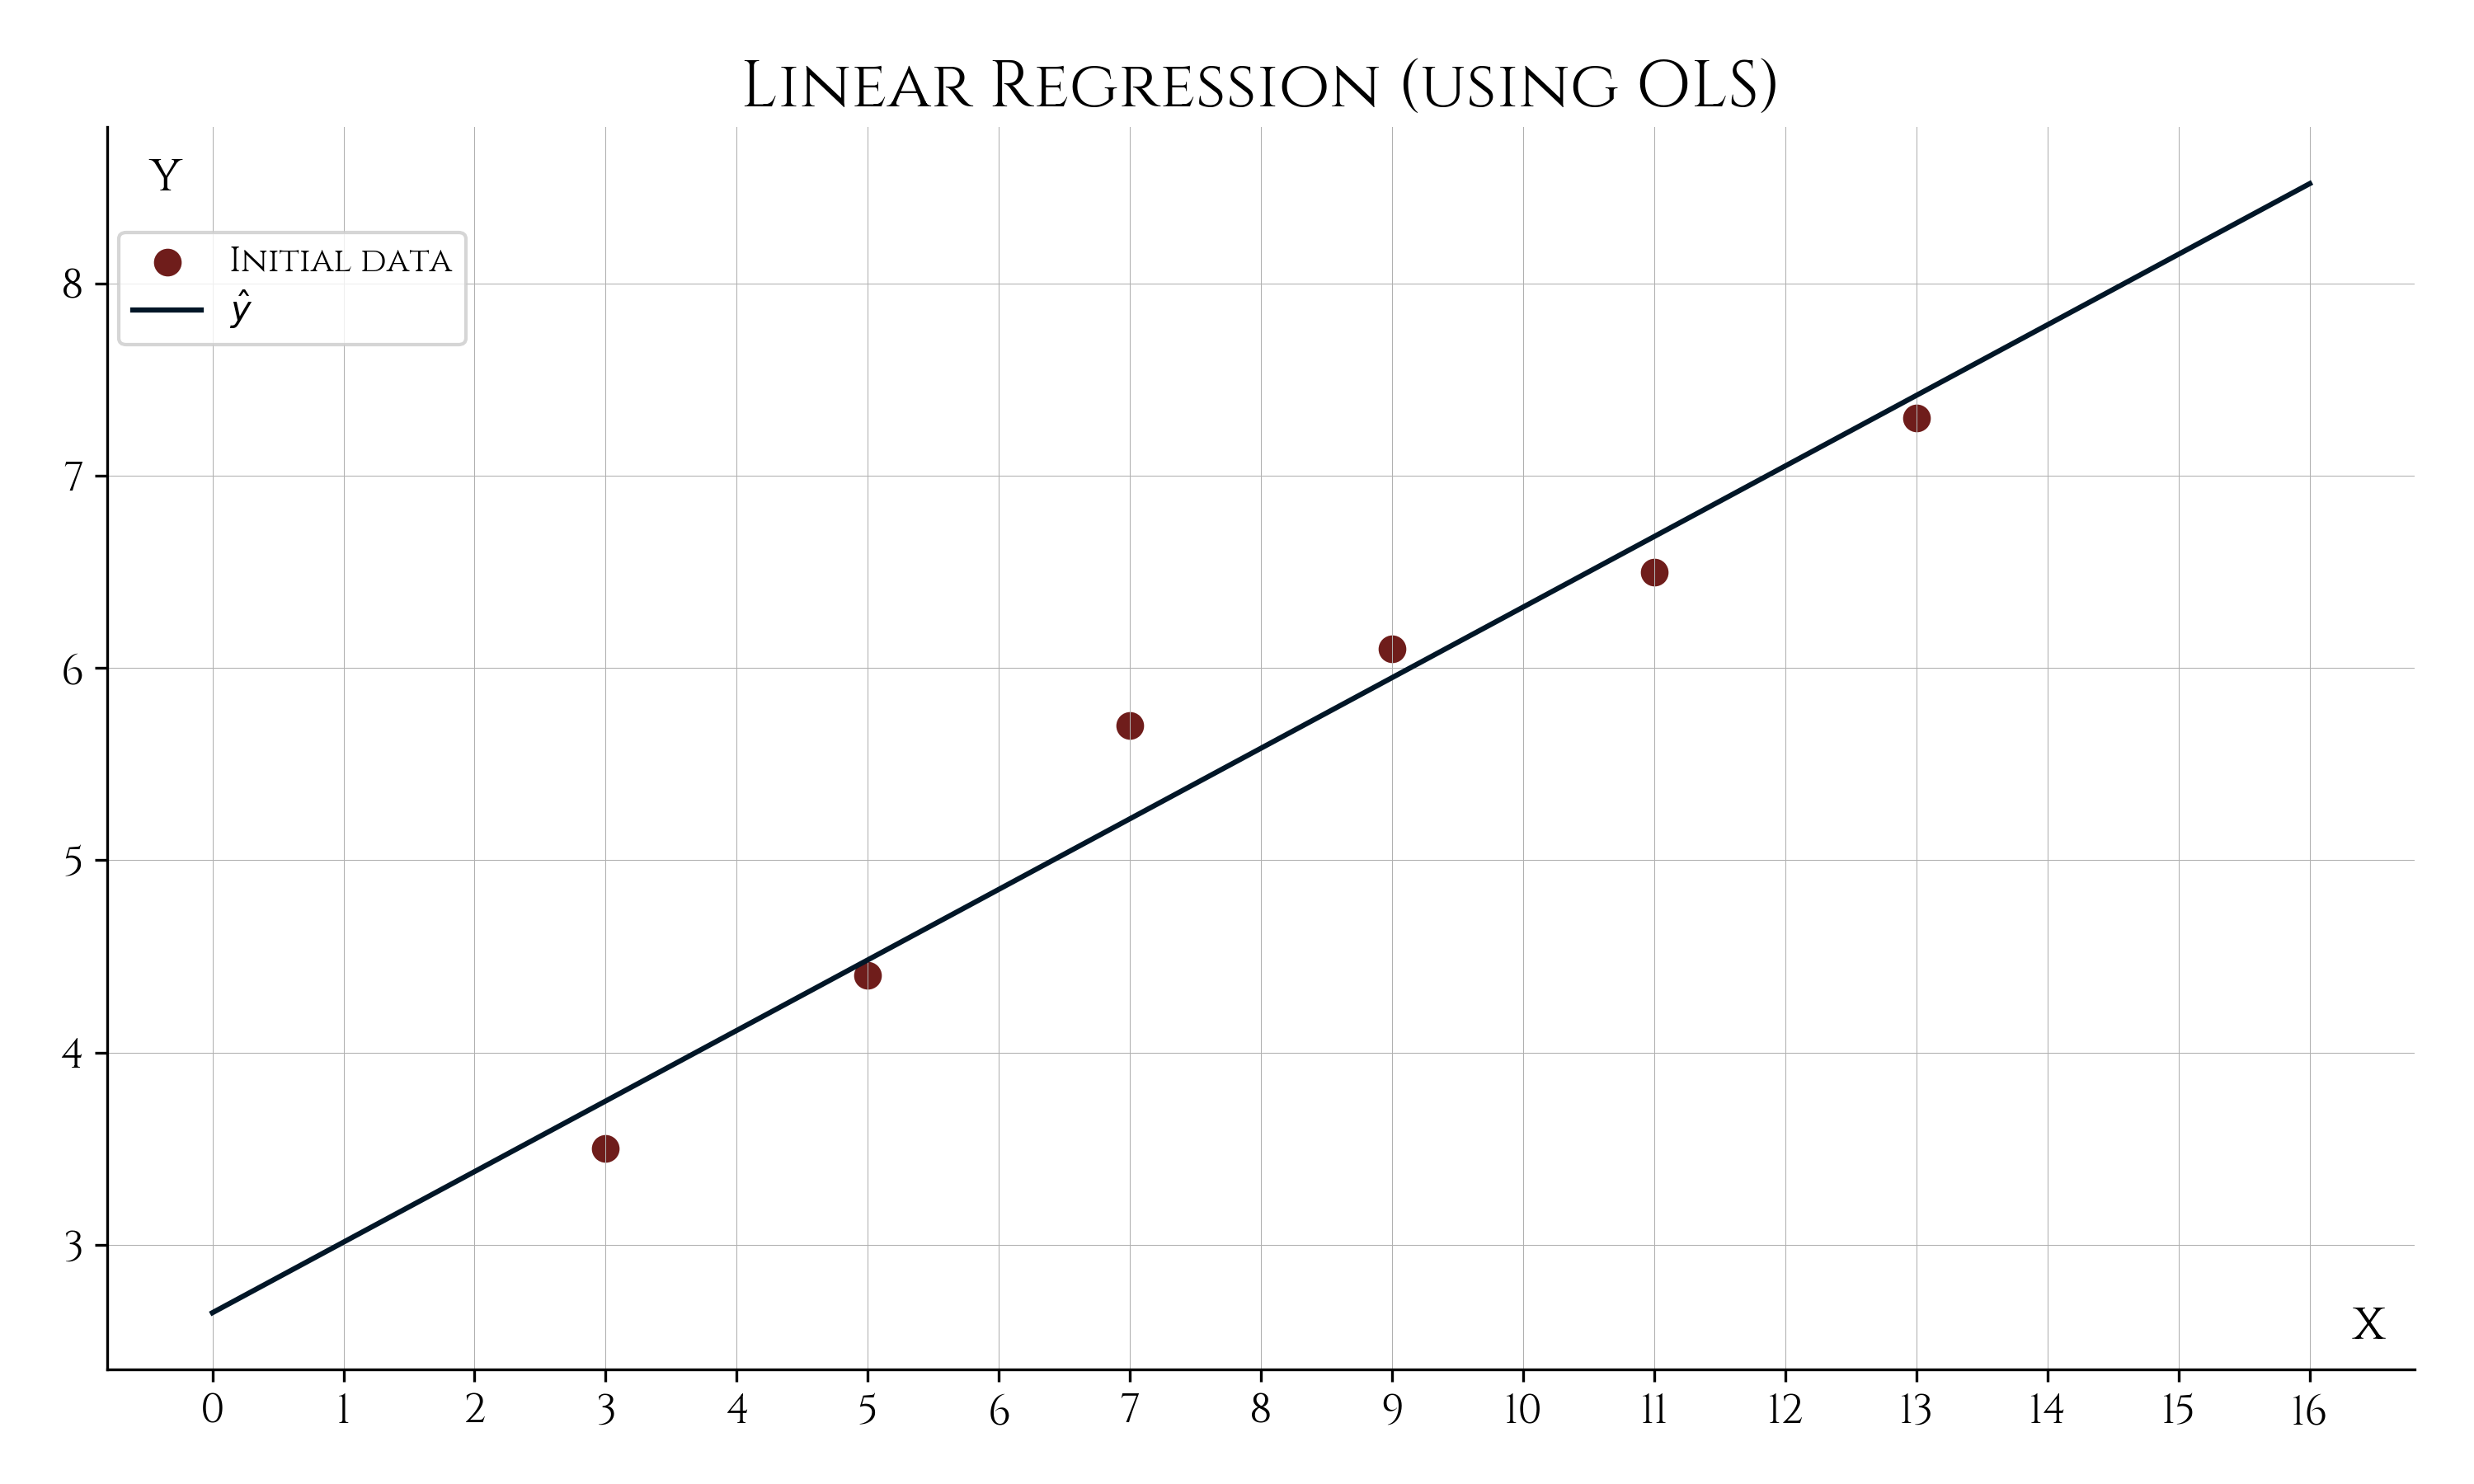
\includegraphics[width=1\textwidth, height=1\textheight, keepaspectratio]{Linear_Regression_Analytical} \\
\end{center}

Что очень похоже на график, подобранный вручную.

\subsubsection*{{Полиномиальная регрессия}}\vspace{-20pt}\rule{\linewidth}{0.1mm}
\addcontentsline{toc}{subsubsection}{Полиномиальная регрессия}

Теперь аналитически выразим формулы для коэффициентов полиномиальной регрессии методом МНК в общем 
случае.

\vfill

\begin{equation*}
    \scalebox{1.5}{
        $\downarrow$
    }
\end{equation*}

\vfill\newpage

\begin{center}
    \fbox{\includegraphics[width=1\textwidth, height=1\textheight, keepaspectratio]{Analyitcal_Polynomial_Regression_1}} \\
\end{center}

\begin{center}
    \fbox{\includegraphics[width=1\textwidth, height=1\textheight, keepaspectratio]{Analyitcal_Polynomial_Regression_2}} \\
\end{center}

\begin{center}
    \fbox{\includegraphics[width=1\textwidth, height=1\textheight, keepaspectratio]{Analyitcal_Polynomial_Regression_3}} \\
\end{center}

\newpage

Тепер вычислим коэффиценты для случая n = 3.

\begin{center}
    \begin{lstlisting}[language=Python]
overlineX,  overlineX2, overlineX3, \
overlineX4, overlineX5, overlineX6 = \
        sympy.symbols('\\overline{X} \\overline{X^2} \\overline{X^3} \\overline{X^4} \\overline{X^5} \\overline{X^6}')
beta0, beta1, \
beta2, beta3 = \
        sympy.symbols('\\hat{\\beta_0} \\hat{\\beta_1} \\hat{\\beta_2} \\hat{\\beta_3}')
overlineY,   overlineXY, \
overlineX2Y, overlineX3Y = \
        sympy.symbols('\\overline{Y} \\overline{XY} \\overline{X^2Y} \\overline{X^3Y}')

X = sympy.Matrix([[1,          overlineX,  overlineX2, overlineX3], 
                  [overlineX,  overlineX2, overlineX3, overlineX4],
                  [overlineX2, overlineX3, overlineX4, overlineX5],
                  [overlineX3, overlineX4, overlineX5, overlineX6]])
b = sympy.Matrix([beta0, beta1, beta2, beta3])
Y = sympy.Matrix([overlineY, overlineXY, overlineX2Y, overlineX3Y])

print(f'$$ b = {sympy.latex(X)}^{{-1}} {sympy.latex(Y)} $$')
display(Latex(f'$$ b = {sympy.latex(X)}^{{-1}} {sympy.latex(Y)} $$'))
    \end{lstlisting}
\end{center}

\begin{equation*}
    b = \left[\begin{matrix}1 & \overline{X} & \overline{X^2} & \overline{X^3}\\\overline{X} & \overline{X^2} & \overline{X^3} & \overline{X^4}\\\overline{X^2} & \overline{X^3} & \overline{X^4} & \overline{X^5}\\\overline{X^3} & \overline{X^4} & \overline{X^5} & \overline{X^6}\end{matrix}\right]^{-1} \left[\begin{matrix}\overline{Y}\\\overline{XY}\\\overline{X^2Y}\\\overline{X^3Y}\end{matrix}\right]
\end{equation*}

\begin{center}
    \begin{lstlisting}[language=Python]
b = X.inv() * Y

print(f'$$ b = {sympy.latex(X)}^{{-1}} {sympy.latex(Y)} $$')
display(Latex(f'$$ {sympy.latex(b)} $$'))
    \end{lstlisting}
\end{center}

Выведем часть полученного вектора в общем виде для случае (n=3):

\[
\scalebox{0.5}{
$\left[\begin{matrix}\frac{\overline{XY} \left(- \overline{X^2} \overline{X^3} \overline{X^6} + \overline{X^2} \overline{X^4} \overline{X^5} + \left(\overline{X^3}\right)^{2} \overline{X^5} - \overline{X^3} \left(\overline{X^4}\right)^{2} + \overline{X^4} \overline{X^6} \overline{X} - \left(\overline{X^5}\right)^{2} \overline{X}\right)}{\left(\overline{X^2}\right)^{3} \overline{X^6} - 2 \left(\overline{X^2}\right)^{2} \overline{X^3} \overline{X^5} - \left(\overline{X^2}\right)^{2} \left(\overline{X^4}\right)^{2} + 3 \overline{X^2} \left(\overline{X^3}\right)^{2} \overline{X^4} - 2 \overline{X^2} \overline{X^3} \overline{X^6} \overline{X} + 2 \overline{X^2} \overline{X^4} \overline{X^5} \overline{X} - \overline{X^2} \overline{X^4} \overline{X^6} + \overline{X^2} \left(\overline{X^5}\right)^{2} - \left(\overline{X^3}\right)^{4} + 2 \left(\overline{X^3}\right)^{2} \overline{X^5} \overline{X} + \left(\overline{X^3}\right)^{2} \overline{X^6} - 2 \overline{X^3} \left(\overline{X^4}\right)^{2} \overline{X} - 2 \overline{X^3} \overline{X^4} \overline{X^5} + \left(\overline{X^4}\right)^{3} + \overline{X^4} \overline{X^6} \overline{X}^{2} - \left(\overline{X^5}\right)^{2} \overline{X}^{2}} + \frac{\overline{X^2Y} \left(\left(\overline{X^2}\right)^{2} \overline{X^6} - \overline{X^2} \overline{X^3} \overline{X^5} - \overline{X^2} \left(\overline{X^4}\right)^{2} + \left(\overline{X^3}\right)^{2} \overline{X^4} - \overline{X^3} \overline{X^6} \overline{X} + \overline{X^4} \overline{X^5} \overline{X}\right)}{\left(\overline{X^2}\right)^{3} \overline{X^6} - 2 \left(\overline{X^2}\right)^{2} \overline{X^3} \overline{X^5} - \left(\overline{X^2}\right)^{2} \left(\overline{X^4}\right)^{2} + 3 \overline{X^2} \left(\overline{X^3}\right)^{2} \overline{X^4} - 2 \overline{X^2} \overline{X^3} \overline{X^6} \overline{X} + 2 \overline{X^2} \overline{X^4} \overline{X^5} \overline{X} - \overline{X^2} \overline{X^4} \overline{X^6} + \overline{X^2} \left(\overline{X^5}\right)^{2} - \left(\overline{X^3}\right)^{4} + 2 \left(\overline{X^3}\right)^{2} \overline{X^5} \overline{X} + \left(\overline{X^3}\right)^{2} \overline{X^6} - 2 \overline{X^3} \left(\overline{X^4}\right)^{2} \overline{X} - 2 \overline{X^3} \overline{X^4} \overline{X^5} + \left(\overline{X^4}\right)^{3} + \overline{X^4} \overline{X^6} \overline{X}^{2} - \left(\overline{X^5}\right)^{2} \overline{X}^{2}} + \frac{\overline{X^3Y} \left(- \left(\overline{X^2}\right)^{2} \overline{X^5} + 2 \overline{X^2} \overline{X^3} \overline{X^4} - \left(\overline{X^3}\right)^{3} + \overline{X^3} \overline{X^5} \overline{X} - \left(\overline{X^4}\right)^{2} \overline{X}\right)}{\left(\overline{X^2}\right)^{3} \overline{X^6} - 2 \left(\overline{X^2}\right)^{2} \overline{X^3} \overline{X^5} - \left(\overline{X^2}\right)^{2} \left(\overline{X^4}\right)^{2} + 3 \overline{X^2} \left(\overline{X^3}\right)^{2} \overline{X^4} - 2 \overline{X^2} \overline{X^3} \overline{X^6} \overline{X} + 2 \overline{X^2} \overline{X^4} \overline{X^5} \overline{X} - \overline{X^2} \overline{X^4} \overline{X^6} + \overline{X^2} \left(\overline{X^5}\right)^{2} - \left(\overline{X^3}\right)^{4} + 2 \left(\overline{X^3}\right)^{2} \overline{X^5} \overline{X} + \left(\overline{X^3}\right)^{2} \overline{X^6} - 2 \overline{X^3} \left(\overline{X^4}\right)^{2} \overline{X} - 2 \overline{X^3} \overline{X^4} \overline{X^5} + \left(\overline{X^4}\right)^{3} + \overline{X^4} \overline{X^6} \overline{X}^{2} - \left(\overline{X^5}\right)^{2} \overline{X}^{2}} + \frac{\overline{Y} \left(- \overline{X^2} \overline{X^4} \overline{X^6} + \overline{X^2} \left(\overline{X^5}\right)^{2} + \left(\overline{X^3}\right)^{2} \overline{X^6} - 2 \overline{X^3} \overline{X^4} \overline{X^5} + \left(\overline{X^4}\right)^{3}\right)}{\left(\overline{X^2}\right)^{3} \overline{X^6} - 2 \left(\overline{X^2}\right)^{2} \overline{X^3} \overline{X^5} - \left(\overline{X^2}\right)^{2} \left(\overline{X^4}\right)^{2} + 3 \overline{X^2} \left(\overline{X^3}\right)^{2} \overline{X^4} - 2 \overline{X^2} \overline{X^3} \overline{X^6} \overline{X} + 2 \overline{X^2} \overline{X^4} \overline{X^5} \overline{X} - \overline{X^2} \overline{X^4} \overline{X^6} + \overline{X^2} \left(\overline{X^5}\right)^{2} - \left(\overline{X^3}\right)^{4} + 2 \left(\overline{X^3}\right)^{2} \overline{X^5} \overline{X} + \left(\overline{X^3}\right)^{2} \overline{X^6} - 2 \overline{X^3} \left(\overline{X^4}\right)^{2} \overline{X} - 2 \overline{X^3} \overline{X^4} \overline{X^5} + \left(\overline{X^4}\right)^{3} + \overline{X^4} \overline{X^6} \overline{X}^{2} - \left(\overline{X^5}\right)^{2} \overline{X}^{2}}\\\frac{\overline{XY} \left(\left(\overline{X^2}\right)^{2} \overline{X^6} - 2 \overline{X^2} \overline{X^3} \overline{X^5} + \left(\overline{X^3}\right)^{2} \overline{X^4} - \overline{X^4} \overline{X^6} + \left(\overline{X^5}\right)^{2}\right)}{\left(\overline{X^2}\right)^{3} \overline{X^6} - 2 \left(\overline{X^2}\right)^{2} \overline{X^3} \overline{X^5} - \left(\overline{X^2}\right)^{2} \left(\overline{X^4}\right)^{2} + 3 \overline{X^2} \left(\overline{X^3}\right)^{2} \overline{X^4} - 2 \overline{X^2} \overline{X^3} \overline{X^6} \overline{X} + 2 \overline{X^2} \overline{X^4} \overline{X^5} \overline{X} - \overline{X^2} \overline{X^4} \overline{X^6} + \overline{X^2} \left(\overline{X^5}\right)^{2} - \left(\overline{X^3}\right)^{4} + 2 \left(\overline{X^3}\right)^{2} \overline{X^5} \overline{X} + \left(\overline{X^3}\right)^{2} \overline{X^6} - 2 \overline{X^3} \left(\overline{X^4}\right)^{2} \overline{X} - 2 \overline{X^3} \overline{X^4} \overline{X^5} + \left(\overline{X^4}\right)^{3} + \overline{X^4} \overline{X^6} \overline{X}^{2} - \left(\overline{X^5}\right)^{2} \overline{X}^{2}} + \frac{\overline{X^2Y} \left(\overline{X^2} \overline{X^3} \overline{X^4} - \overline{X^2} \overline{X^6} \overline{X} - \left(\overline{X^3}\right)^{3} + \overline{X^3} \overline{X^5} \overline{X} + \overline{X^3} \overline{X^6} - \overline{X^4} \overline{X^5}\right)}{\left(\overline{X^2}\right)^{3} \overline{X^6} - 2 \left(\overline{X^2}\right)^{2} \overline{X^3} \overline{X^5} - \left(\overline{X^2}\right)^{2} \left(\overline{X^4}\right)^{2} + 3 \overline{X^2} \left(\overline{X^3}\right)^{2} \overline{X^4} - 2 \overline{X^2} \overline{X^3} \overline{X^6} \overline{X} + 2 \overline{X^2} \overline{X^4} \overline{X^5} \overline{X} - \overline{X^2} \overline{X^4} \overline{X^6} + \overline{X^2} \left(\overline{X^5}\right)^{2} - \left(\overline{X^3}\right)^{4} + 2 \left(\overline{X^3}\right)^{2} \overline{X^5} \overline{X} + \left(\overline{X^3}\right)^{2} \overline{X^6} - 2 \overline{X^3} \left(\overline{X^4}\right)^{2} \overline{X} - 2 \overline{X^3} \overline{X^4} \overline{X^5} + \left(\overline{X^4}\right)^{3} + \overline{X^4} \overline{X^6} \overline{X}^{2} - \left(\overline{X^5}\right)^{2} \overline{X}^{2}} + \frac{\overline{X^3Y} \left(- \left(\overline{X^2}\right)^{2} \overline{X^4} + \overline{X^2} \left(\overline{X^3}\right)^{2} + \overline{X^2} \overline{X^5} \overline{X} - \overline{X^3} \overline{X^4} \overline{X} - \overline{X^3} \overline{X^5} + \left(\overline{X^4}\right)^{2}\right)}{\left(\overline{X^2}\right)^{3} \overline{X^6} - 2 \left(\overline{X^2}\right)^{2} \overline{X^3} \overline{X^5} - \left(\overline{X^2}\right)^{2} \left(\overline{X^4}\right)^{2} + 3 \overline{X^2} \left(\overline{X^3}\right)^{2} \overline{X^4} - 2 \overline{X^2} \overline{X^3} \overline{X^6} \overline{X} + 2 \overline{X^2} \overline{X^4} \overline{X^5} \overline{X} - \overline{X^2} \overline{X^4} \overline{X^6} + \overline{X^2} \left(\overline{X^5}\right)^{2} - \left(\overline{X^3}\right)^{4} + 2 \left(\overline{X^3}\right)^{2} \overline{X^5} \overline{X} + \left(\overline{X^3}\right)^{2} \overline{X^6} - 2 \overline{X^3} \left(\overline{X^4}\right)^{2} \overline{X} - 2 \overline{X^3} \overline{X^4} \overline{X^5} + \left(\overline{X^4}\right)^{3} + \overline{X^4} \overline{X^6} \overline{X}^{2} - \left(\overline{X^5}\right)^{2} \overline{X}^{2}} + \frac{\overline{Y} \left(- \overline{X^2} \overline{X^3} \overline{X^6} + \overline{X^2} \overline{X^4} \overline{X^5} + \left(\overline{X^3}\right)^{2} \overline{X^5} - \overline{X^3} \left(\overline{X^4}\right)^{2} + \overline{X^4} \overline{X^6} \overline{X} - \left(\overline{X^5}\right)^{2} \overline{X}\right)}{\left(\overline{X^2}\right)^{3} \overline{X^6} - 2 \left(\overline{X^2}\right)^{2} \overline{X^3} \overline{X^5} - \left(\overline{X^2}\right)^{2} \left(\overline{X^4}\right)^{2} + 3 \overline{X^2} \left(\overline{X^3}\right)^{2} \overline{X^4} - 2 \overline{X^2} \overline{X^3} \overline{X^6} \overline{X} + 2 \overline{X^2} \overline{X^4} \overline{X^5} \overline{X} - \overline{X^2} \overline{X^4} \overline{X^6} + \overline{X^2} \left(\overline{X^5}\right)^{2} - \left(\overline{X^3}\right)^{4} + 2 \left(\overline{X^3}\right)^{2} \overline{X^5} \overline{X} + \left(\overline{X^3}\right)^{2} \overline{X^6} - 2 \overline{X^3} \left(\overline{X^4}\right)^{2} \overline{X} - 2 \overline{X^3} \overline{X^4} \overline{X^5} + \left(\overline{X^4}\right)^{3} + \overline{X^4} \overline{X^6} \overline{X}^{2} - \left(\overline{X^5}\right)^{2} \overline{X}^{2}}\\\frac{\overline{XY} \left(\overline{X^2} \overline{X^3} \overline{X^4} - \overline{X^2} \overline{X^6} \overline{X} - \left(\overline{X^3}\right)^{3} + \overline{X^3} \overline{X^5} \overline{X} + \overline{X^3} \overline{X^6} - \overline{X^4} \overline{X^5}\right)}{\left(\overline{X^2}\right)^{3} \overline{X^6} - 2 \left(\overline{X^2}\right)^{2} \overline{X^3} \overline{X^5} - \left(\overline{X^2}\right)^{2} \left(\overline{X^4}\right)^{2} + 3 \overline{X^2} \left(\overline{X^3}\right)^{2} \overline{X^4} - 2 \overline{X^2} \overline{X^3} \overline{X^6} \overline{X} + 2 \overline{X^2} \overline{X^4} \overline{X^5} \overline{X} - \overline{X^2} \overline{X^4} \overline{X^6} + \overline{X^2} \left(\overline{X^5}\right)^{2} - \left(\overline{X^3}\right)^{4} + 2 \left(\overline{X^3}\right)^{2} \overline{X^5} \overline{X} + \left(\overline{X^3}\right)^{2} \overline{X^6} - 2 \overline{X^3} \left(\overline{X^4}\right)^{2} \overline{X} - 2 \overline{X^3} \overline{X^4} \overline{X^5} + \left(\overline{X^4}\right)^{3} + \overline{X^4} \overline{X^6} \overline{X}^{2} - \left(\overline{X^5}\right)^{2} \overline{X}^{2}} + \frac{\overline{X^2Y} \left(\overline{X^2} \left(\overline{X^3}\right)^{2} - \overline{X^2} \overline{X^6} - 2 \overline{X^3} \overline{X^4} \overline{X} + \left(\overline{X^4}\right)^{2} + \overline{X^6} \overline{X}^{2}\right)}{\left(\overline{X^2}\right)^{3} \overline{X^6} - 2 \left(\overline{X^2}\right)^{2} \overline{X^3} \overline{X^5} - \left(\overline{X^2}\right)^{2} \left(\overline{X^4}\right)^{2} + 3 \overline{X^2} \left(\overline{X^3}\right)^{2} \overline{X^4} - 2 \overline{X^2} \overline{X^3} \overline{X^6} \overline{X} + 2 \overline{X^2} \overline{X^4} \overline{X^5} \overline{X} - \overline{X^2} \overline{X^4} \overline{X^6} + \overline{X^2} \left(\overline{X^5}\right)^{2} - \left(\overline{X^3}\right)^{4} + 2 \left(\overline{X^3}\right)^{2} \overline{X^5} \overline{X} + \left(\overline{X^3}\right)^{2} \overline{X^6} - 2 \overline{X^3} \left(\overline{X^4}\right)^{2} \overline{X} - 2 \overline{X^3} \overline{X^4} \overline{X^5} + \left(\overline{X^4}\right)^{3} + \overline{X^4} \overline{X^6} \overline{X}^{2} - \left(\overline{X^5}\right)^{2} \overline{X}^{2}} + \frac{\overline{X^3Y} \left(- \left(\overline{X^2}\right)^{2} \overline{X^3} + \overline{X^2} \overline{X^4} \overline{X} + \overline{X^2} \overline{X^5} + \left(\overline{X^3}\right)^{2} \overline{X} - \overline{X^3} \overline{X^4} - \overline{X^5} \overline{X}^{2}\right)}{\left(\overline{X^2}\right)^{3} \overline{X^6} - 2 \left(\overline{X^2}\right)^{2} \overline{X^3} \overline{X^5} - \left(\overline{X^2}\right)^{2} \left(\overline{X^4}\right)^{2} + 3 \overline{X^2} \left(\overline{X^3}\right)^{2} \overline{X^4} - 2 \overline{X^2} \overline{X^3} \overline{X^6} \overline{X} + 2 \overline{X^2} \overline{X^4} \overline{X^5} \overline{X} - \overline{X^2} \overline{X^4} \overline{X^6} + \overline{X^2} \left(\overline{X^5}\right)^{2} - \left(\overline{X^3}\right)^{4} + 2 \left(\overline{X^3}\right)^{2} \overline{X^5} \overline{X} + \left(\overline{X^3}\right)^{2} \overline{X^6} - 2 \overline{X^3} \left(\overline{X^4}\right)^{2} \overline{X} - 2 \overline{X^3} \overline{X^4} \overline{X^5} + \left(\overline{X^4}\right)^{3} + \overline{X^4} \overline{X^6} \overline{X}^{2} - \left(\overline{X^5}\right)^{2} \overline{X}^{2}} + \frac{\overline{Y} \left(\left(\overline{X^2}\right)^{2} \overline{X^6} - \overline{X^2} \overline{X^3} \overline{X^5} - \overline{X^2} \left(\overline{X^4}\right)^{2} + \left(\overline{X^3}\right)^{2} \overline{X^4} - \overline{X^3} \overline{X^6} \overline{X} + \overline{X^4} \overline{X^5} \overline{X}\right)}{\left(\overline{X^2}\right)^{3} \overline{X^6} - 2 \left(\overline{X^2}\right)^{2} \overline{X^3} \overline{X^5} - \left(\overline{X^2}\right)^{2} \left(\overline{X^4}\right)^{2} + 3 \overline{X^2} \left(\overline{X^3}\right)^{2} \overline{X^4} - 2 \overline{X^2} \overline{X^3} \overline{X^6} \overline{X} + 2 \overline{X^2} \overline{X^4} \overline{X^5} \overline{X} - \overline{X^2} \overline{X^4} \overline{X^6} + \overline{X^2} \left(\overline{X^5}\right)^{2} - \left(\overline{X^3}\right)^{4} + 2 \left(\overline{X^3}\right)^{2} \overline{X^5} \overline{X} + \left(\overline{X^3}\right)^{2} \overline{X^6} - 2 \overline{X^3} \left(\overline{X^4}\right)^{2} \overline{X} - 2 \overline{X^3} \overline{X^4} \overline{X^5} + \left(\overline{X^4}\right)^{3} + \overline{X^4} \overline{X^6} \overline{X}^{2} - \left(\overline{X^5}\right)^{2} \overline{X}^{2}}\\\frac{\overline{XY} \left(- \left(\overline{X^2}\right)^{2} \overline{X^4} + \overline{X^2} \left(\overline{X^3}\right)^{2} + \overline{X^2} \overline{X^5} \overline{X} - \overline{X^3} \overline{X^4} \overline{X} - \overline{X^3} \overline{X^5} + \left(\overline{X^4}\right)^{2}\right)}{\left(\overline{X^2}\right)^{3} \overline{X^6} - 2 \left(\overline{X^2}\right)^{2} \overline{X^3} \overline{X^5} - \left(\overline{X^2}\right)^{2} \left(\overline{X^4}\right)^{2} + 3 \overline{X^2} \left(\overline{X^3}\right)^{2} \overline{X^4} - 2 \overline{X^2} \overline{X^3} \overline{X^6} \overline{X} + 2 \overline{X^2} \overline{X^4} \overline{X^5} \overline{X} - \overline{X^2} \overline{X^4} \overline{X^6} + \overline{X^2} \left(\overline{X^5}\right)^{2} - \left(\overline{X^3}\right)^{4} + 2 \left(\overline{X^3}\right)^{2} \overline{X^5} \overline{X} + \left(\overline{X^3}\right)^{2} \overline{X^6} - 2 \overline{X^3} \left(\overline{X^4}\right)^{2} \overline{X} - 2 \overline{X^3} \overline{X^4} \overline{X^5} + \left(\overline{X^4}\right)^{3} + \overline{X^4} \overline{X^6} \overline{X}^{2} - \left(\overline{X^5}\right)^{2} \overline{X}^{2}} + \frac{\overline{X^2Y} \left(- \left(\overline{X^2}\right)^{2} \overline{X^3} + \overline{X^2} \overline{X^4} \overline{X} + \overline{X^2} \overline{X^5} + \left(\overline{X^3}\right)^{2} \overline{X} - \overline{X^3} \overline{X^4} - \overline{X^5} \overline{X}^{2}\right)}{\left(\overline{X^2}\right)^{3} \overline{X^6} - 2 \left(\overline{X^2}\right)^{2} \overline{X^3} \overline{X^5} - \left(\overline{X^2}\right)^{2} \left(\overline{X^4}\right)^{2} + 3 \overline{X^2} \left(\overline{X^3}\right)^{2} \overline{X^4} - 2 \overline{X^2} \overline{X^3} \overline{X^6} \overline{X} + 2 \overline{X^2} \overline{X^4} \overline{X^5} \overline{X} - \overline{X^2} \overline{X^4} \overline{X^6} + \overline{X^2} \left(\overline{X^5}\right)^{2} - \left(\overline{X^3}\right)^{4} + 2 \left(\overline{X^3}\right)^{2} \overline{X^5} \overline{X} + \left(\overline{X^3}\right)^{2} \overline{X^6} - 2 \overline{X^3} \left(\overline{X^4}\right)^{2} \overline{X} - 2 \overline{X^3} \overline{X^4} \overline{X^5} + \left(\overline{X^4}\right)^{3} + \overline{X^4} \overline{X^6} \overline{X}^{2} - \left(\overline{X^5}\right)^{2} \overline{X}^{2}} + \frac{\overline{X^3Y} \left(\left(\overline{X^2}\right)^{3} - 2 \overline{X^2} \overline{X^3} \overline{X} - \overline{X^2} \overline{X^4} + \left(\overline{X^3}\right)^{2} + \overline{X^4} \overline{X}^{2}\right)}{\left(\overline{X^2}\right)^{3} \overline{X^6} - 2 \left(\overline{X^2}\right)^{2} \overline{X^3} \overline{X^5} - \left(\overline{X^2}\right)^{2} \left(\overline{X^4}\right)^{2} + 3 \overline{X^2} \left(\overline{X^3}\right)^{2} \overline{X^4} - 2 \overline{X^2} \overline{X^3} \overline{X^6} \overline{X} + 2 \overline{X^2} \overline{X^4} \overline{X^5} \overline{X} - \overline{X^2} \overline{X^4} \overline{X^6} + \overline{X^2} \left(\overline{X^5}\right)^{2} - \left(\overline{X^3}\right)^{4} + 2 \left(\overline{X^3}\right)^{2} \overline{X^5} \overline{X} + \left(\overline{X^3}\right)^{2} \overline{X^6} - 2 \overline{X^3} \left(\overline{X^4}\right)^{2} \overline{X} - 2 \overline{X^3} \overline{X^4} \overline{X^5} + \left(\overline{X^4}\right)^{3} + \overline{X^4} \overline{X^6} \overline{X}^{2} - \left(\overline{X^5}\right)^{2} \overline{X}^{2}} + \frac{\overline{Y} \left(- \left(\overline{X^2}\right)^{2} \overline{X^5} + 2 \overline{X^2} \overline{X^3} \overline{X^4} - \left(\overline{X^3}\right)^{3} + \overline{X^3} \overline{X^5} \overline{X} - \left(\overline{X^4}\right)^{2} \overline{X}\right)}{\left(\overline{X^2}\right)^{3} \overline{X^6} - 2 \left(\overline{X^2}\right)^{2} \overline{X^3} \overline{X^5} - \left(\overline{X^2}\right)^{2} \left(\overline{X^4}\right)^{2} + 3 \overline{X^2} \left(\overline{X^3}\right)^{2} \overline{X^4} - 2 \overline{X^2} \overline{X^3} \overline{X^6} \overline{X} + 2 \overline{X^2} \overline{X^4} \overline{X^5} \overline{X} - \overline{X^2} \overline{X^4} \overline{X^6} + \overline{X^2} \left(\overline{X^5}\right)^{2} - \left(\overline{X^3}\right)^{4} + 2 \left(\overline{X^3}\right)^{2} \overline{X^5} \overline{X} + \left(\overline{X^3}\right)^{2} \overline{X^6} - 2 \overline{X^3} \left(\overline{X^4}\right)^{2} \overline{X} - 2 \overline{X^3} \overline{X^4} \overline{X^5} + \left(\overline{X^4}\right)^{3} + \overline{X^4} \overline{X^6} \overline{X}^{2} - \left(\overline{X^5}\right)^{2} \overline{X}^{2}}\end{matrix}\right]$
}
\]

\newpage

Теперь подставим наши данные в данный вектор:

\begin{center}
    \begin{lstlisting}[language=Python]
overlineXn  = lambda n : 1/n_ * sum([x**n for x in x_values_])
overlineXnY = lambda n : 1/n_ * sum([x**n * y for x, y in zip(x_values_, 
                                                              y_values_)])

polynomial_analytical_beta = b.subs([(overlineX,   overlineXn(1)), 
                                     (overlineX2,  overlineXn(2)), 
                                     (overlineX3,  overlineXn(3)), 
                                     (overlineX4,  overlineXn(4)), 
                                     (overlineX5,  overlineXn(5)), 
                                     (overlineX6,  overlineXn(6)),
                                     (overlineY,   overlineXnY(0)),
                                     (overlineXY,  overlineXnY(1)),
                                     (overlineX2Y, overlineXnY(2)),
                                     (overlineX3Y, overlineXnY(3))])

polynomial_analytical_beta
    \end{lstlisting}
\end{center}

Получим:

\begin{equation*}
    \begin{vmatrix}
        0.5933036 \\
        1.196875 \\
        -0.0933036 \\
        0.003125
    \end{vmatrix}
\end{equation*}

Построим график полученной модели:

\begin{center}
    \begin{lstlisting}[language=Python]
polynomial_analytical_func = lambda x: polynomial_analytical_beta[0] + \
                                       polynomial_analytical_beta[1] * x + \
                                       polynomial_analytical_beta[2] * x**2 + \
                                       polynomial_analytical_beta[3] * x**3

new_x_values = np.linspace(0, x_values_[-1] + 3, 100)
new_y_values = polynomial_analytical_func(new_x_values)

y_values_polynomial_analytical = new_y_values

buildBar('Polynomial_Regression_Analytical', 
         '$\\hat{y}$', 
         'Polynomial regression (using OLS, n=3)',
          x_values_, 
          y_values_, 
          new_x_values, 
          new_y_values)
    \end{lstlisting}
\end{center}

Получим:

\begin{center}
    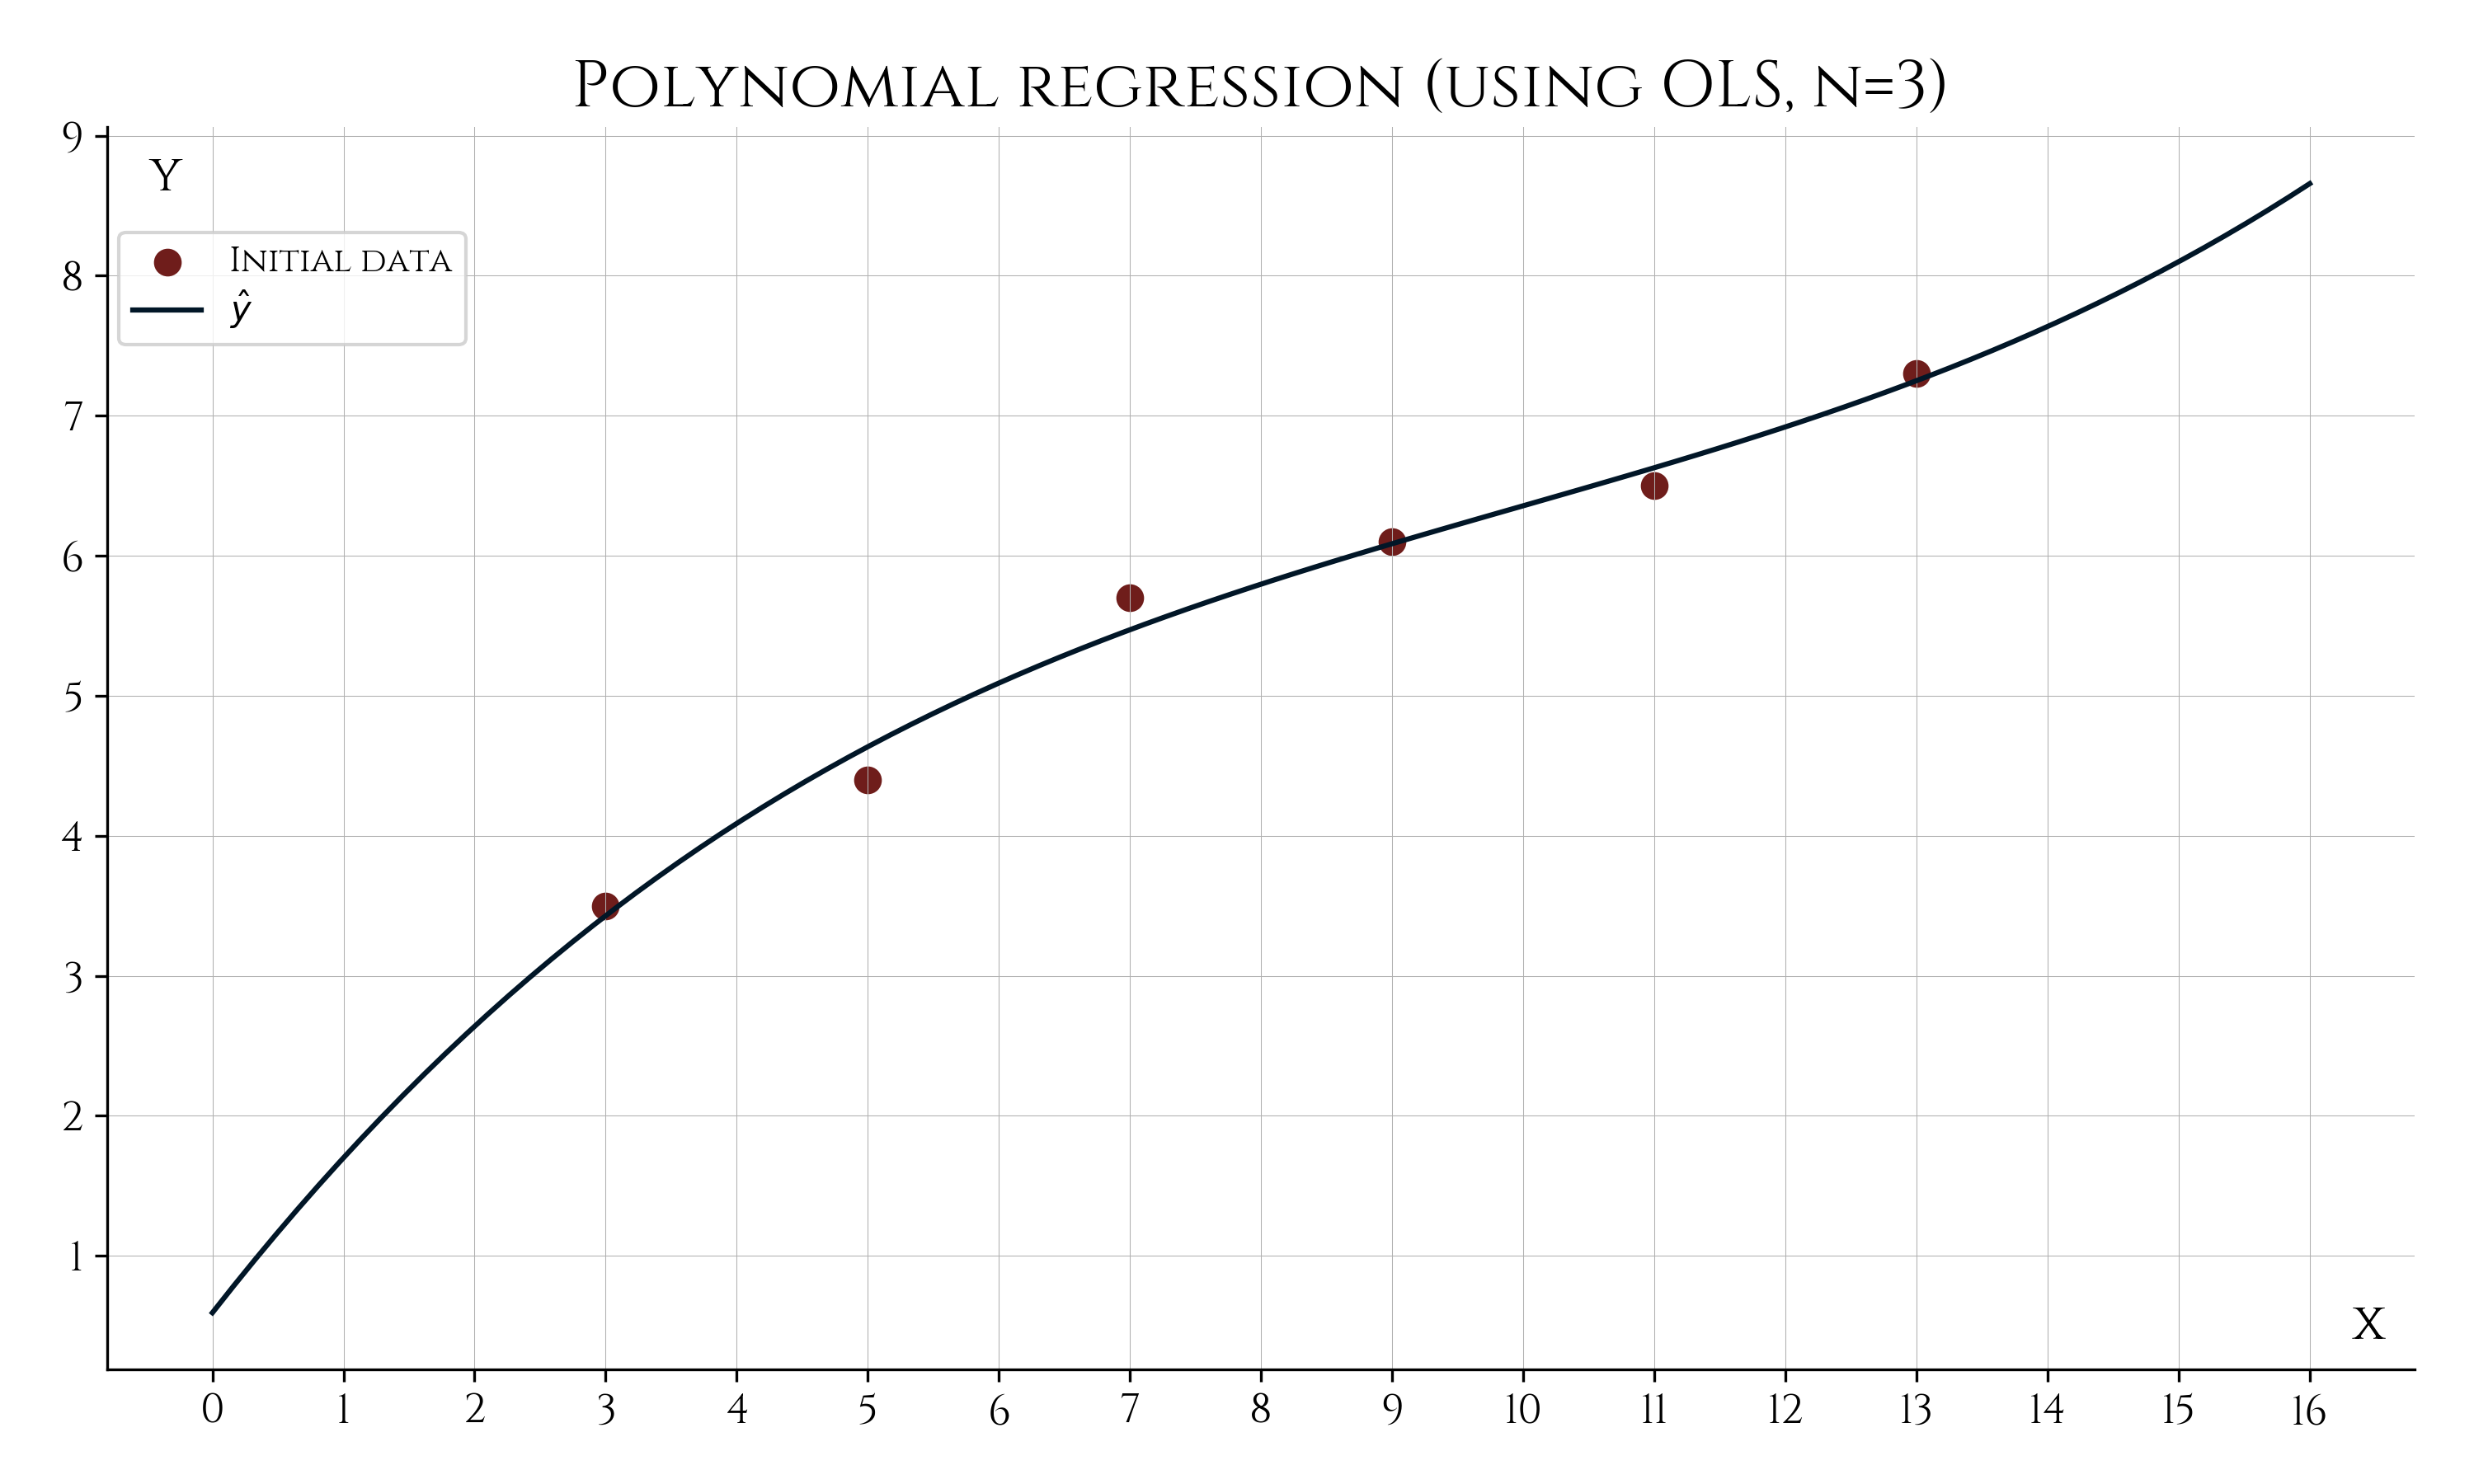
\includegraphics[width=1\textwidth, height=1\textheight, keepaspectratio]{Polynomial_Regression_Analytical} \\
\end{center}

Из графика видно, что данная модель лучше аппроксимирует данные, нежели линейная.

\subsection*{{Часть 4}}\vspace{-20pt}\rule{\linewidth}{0.1mm}
\addcontentsline{toc}{subsection}{Часть 4}

Решить задачу на языке python с использованием библиотеки numpy, привести код, 
привести результат решения. Полученный результат изобразить графически при помощи 
библиотеки matplotlib, привести код для построения значений;

\subsubsection*{{Описание применяемых методов библиотеки}}\vspace{-20pt}\rule{\linewidth}{0.1mm}
\addcontentsline{toc}{subsubsection}{Описание применяемых методов библиотеки}

Воспользуемся следующими методами библиотеки \high{numpy}:

\begin{itemize}
    \item np.array - для создания массива данных
    \item np.ones - для создания массива, заполненного единицами
    \item .T - для транспонирования
    \item np.linalg.inv - для нахождения обратной матрицы
    \item @ - для матричного умножения
    \item np.linspace - для задания сетки
\end{itemize}

\subsubsection*{{Описание хода решения}}
\addcontentsline{toc}{subsubsection}{Описание хода решения}

\paragraph*{{Линейная регрессия}}\vspace{-20pt}\rule{\linewidth}{0.1mm}
\addcontentsline{toc}{paragraph}{Линейная регрессия}

Воспользуемся матричной формой решения:

\begin{equation*}
    \beta = (X^T X)^{-1} X^T Y
\end{equation*}

Реализуем нахождение коэффициентов модели при помощи библиотеки numpy:

\begin{center}
    \begin{lstlisting}[language=Python]
X = np.array([np.ones(n_), np.array(x_values_)]).T
Y = np.array(y_values_).T
linear_numpy_beta = np.linalg.inv((X.T @ X)) @ X.T @ Y

linear_numpy_beta
    \end{lstlisting}
\end{center}

Получим:

\begin{equation*}
    \beta_0 \approx 2.646 \qquad \beta_1 \approx 0.3671
\end{equation*}

Построим график:

\begin{center}
    \begin{lstlisting}[language=Python]
linear_numpy_func = lambda x: linear_numpy_beta[0] + linear_numpy_beta[1] * x

new_x_values = np.linspace(0, x_values_[-1] + 3, 100)
new_y_values = linear_numpy_func(new_x_values)

y_values_linear_numpy = new_y_values

buildBar('Linear_Regression_numpy', 
         '$\\hat{y}$', 
         'Linear Regression (using OLS) with numpy', 
         x_values_, 
         y_values_, 
         new_x_values, 
         new_y_values)
    \end{lstlisting}
\end{center}

\begin{center}
    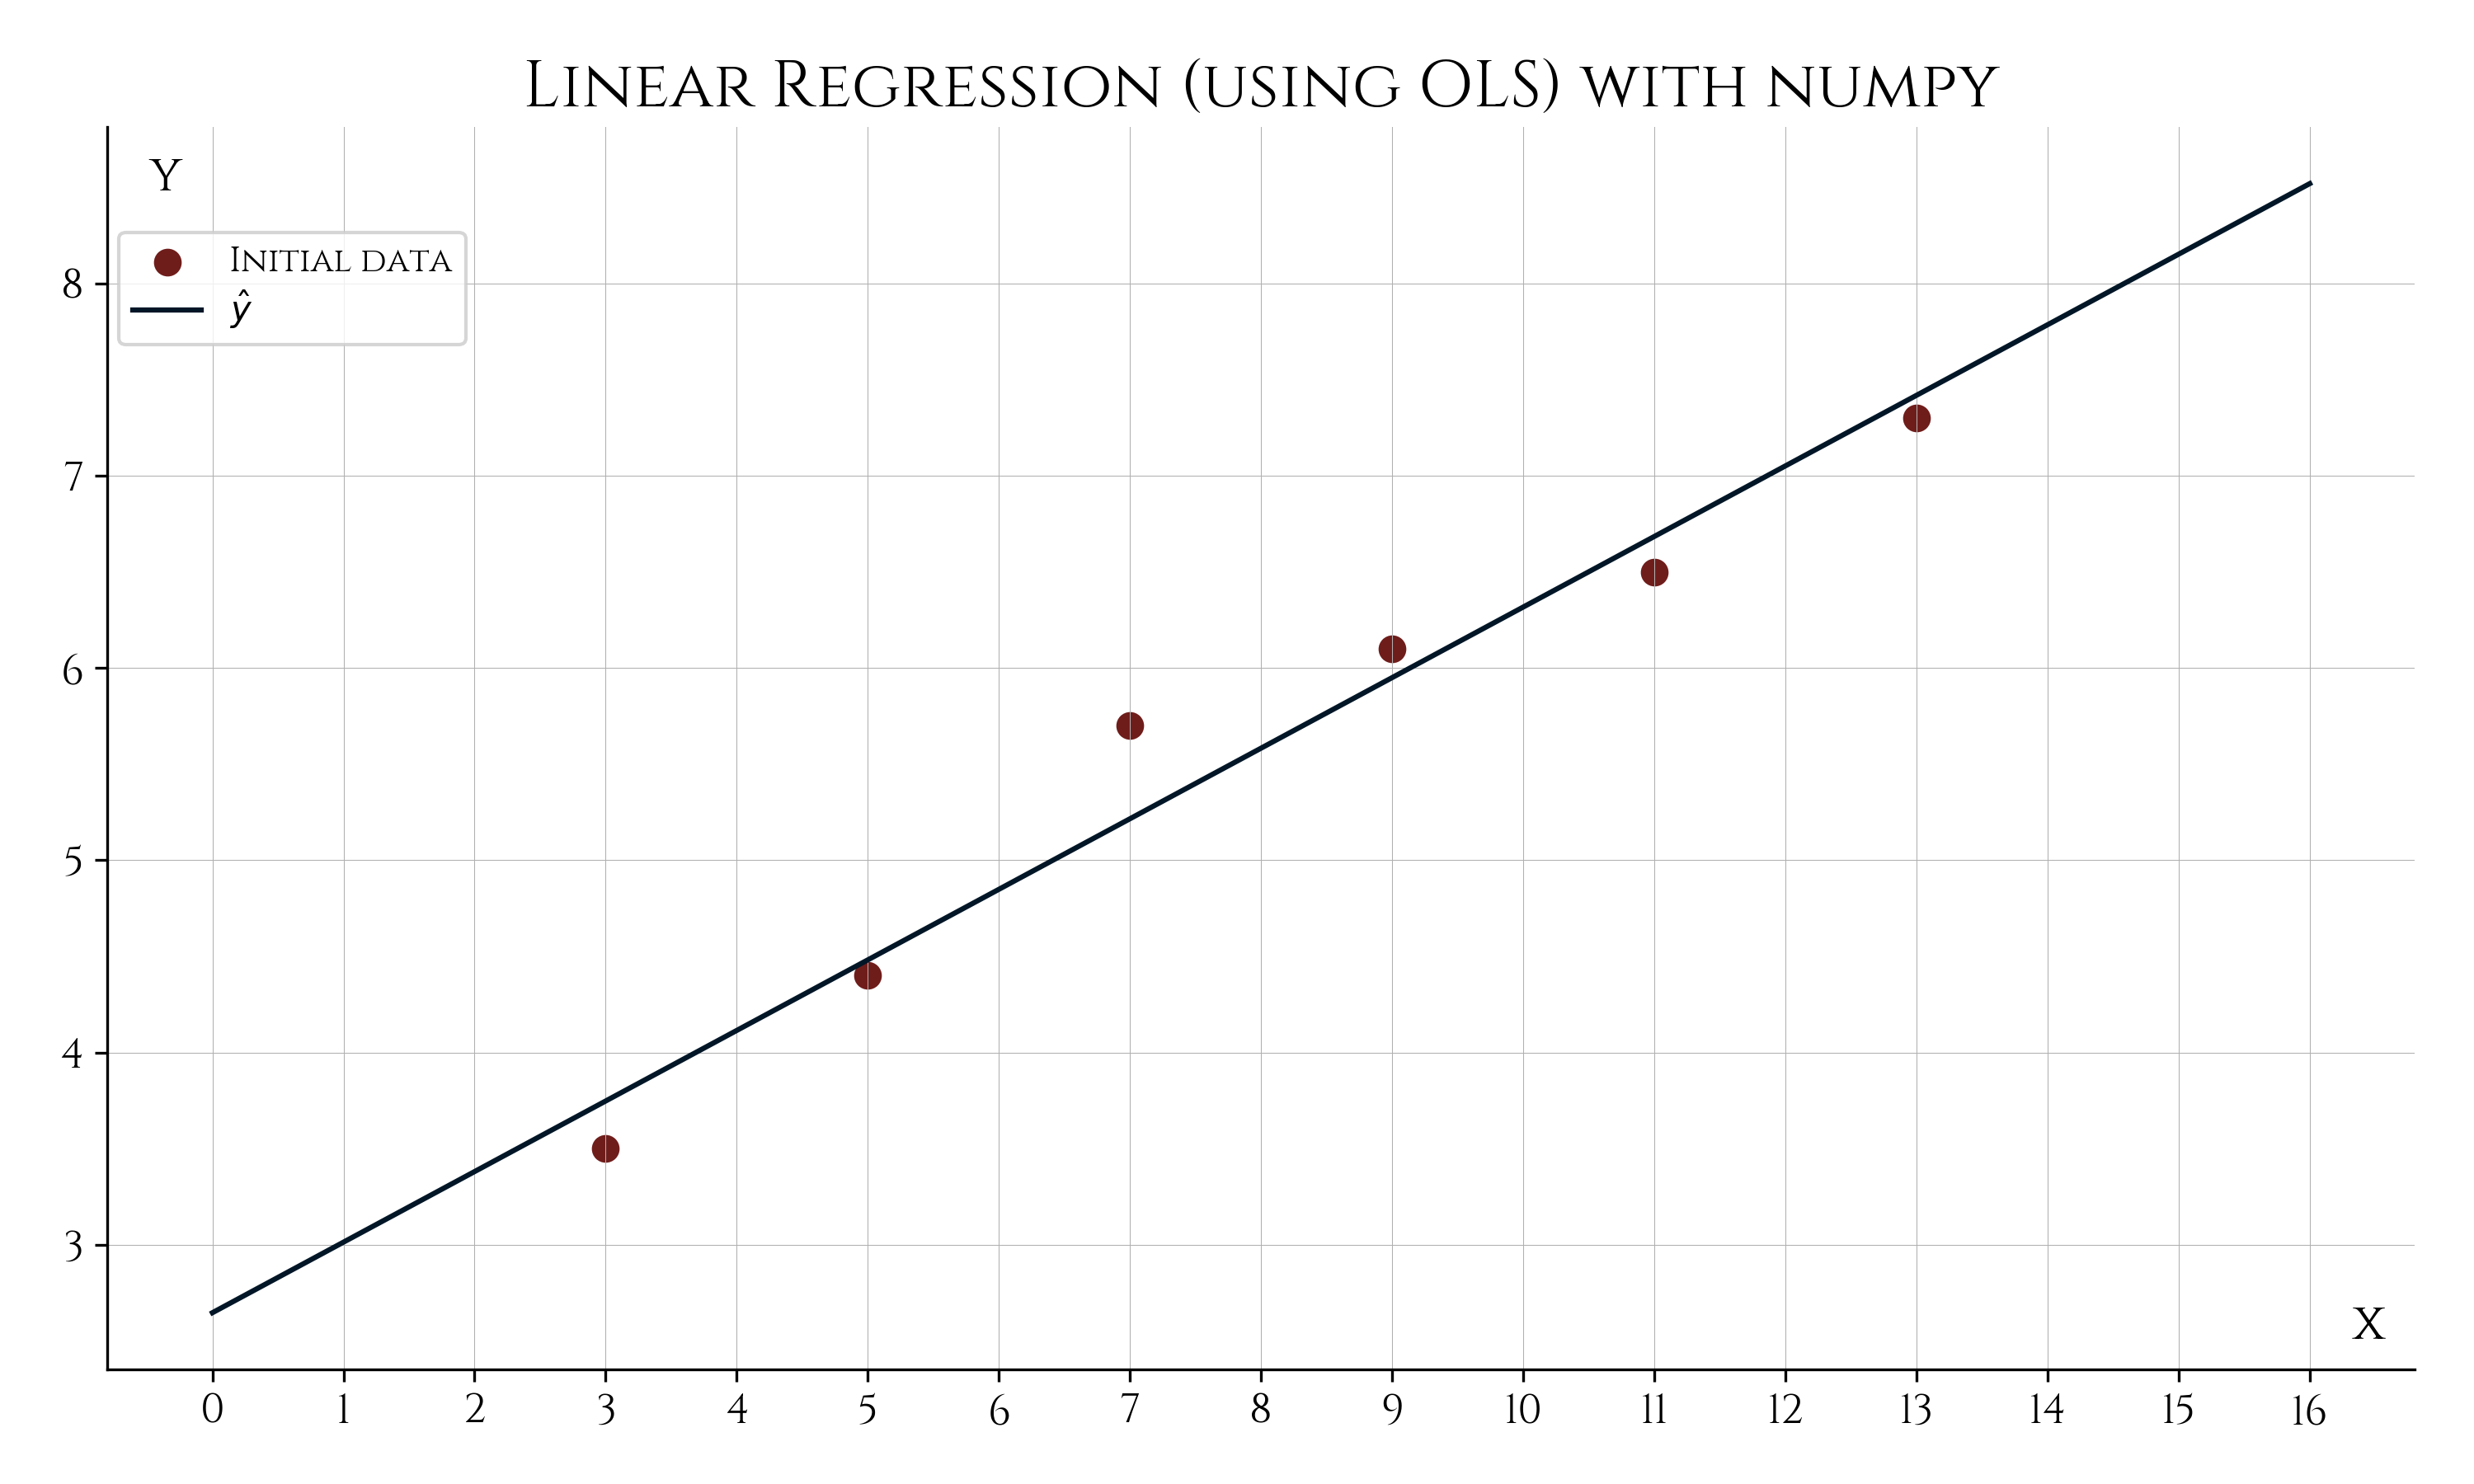
\includegraphics[width=1\textwidth, height=1\textheight, keepaspectratio]{Linear_Regression_numpy} \\
\end{center}

Результаты получились аналогичными тем, что были найдены аналитически.

\paragraph*{{Полиномиальная регрессия}}\vspace{-20pt}\rule{\linewidth}{0.1mm}
\addcontentsline{toc}{paragraph}{Полиномиальная регрессия}

Реализуем нахождение коэффициентов модели при помощи библиотеки numpy:

\begin{center}
    \begin{lstlisting}[language=Python]
X = np.array([np.ones(n_), 
              np.array(x_values_), 
              np.array(x_values_)**2, 
              np.array(x_values_)**3]).T
Y = np.array(y_values_).T
polynomial_numpy_beta = np.linalg.inv((X.T @ X)) @ X.T @ Y

polynomial_numpy_beta
    \end{lstlisting}
\end{center}

Получим:

\begin{equation*}
    \begin{vmatrix}
        0.5933036 \\
        1.196875 \\
        -0.0933036 \\
        0.003125
    \end{vmatrix}
\end{equation*}

Построим график:

\begin{center}
    \begin{lstlisting}[language=Python]
polynomial_numpy_func = lambda x: polynomial_numpy_beta[0] + \
                                  polynomial_numpy_beta[1] * x + \
                                  polynomial_numpy_beta[2] * x**2 + \
                                  polynomial_numpy_beta[3] * x**3

new_x_values = np.linspace(0, x_values_[-1] + 3, 100)
new_y_values = polynomial_numpy_func(new_x_values)

y_values_polynomial_numpy = new_y_values

buildBar('Polynomial_Regression_numpy', 
         '$\\hat{y}$', 
         'Polynomial regression (using OLS, n=3) with numpy', 
         x_values_, 
         y_values_, 
         new_x_values, 
         new_y_values)
    \end{lstlisting}
\end{center}

\begin{center}
    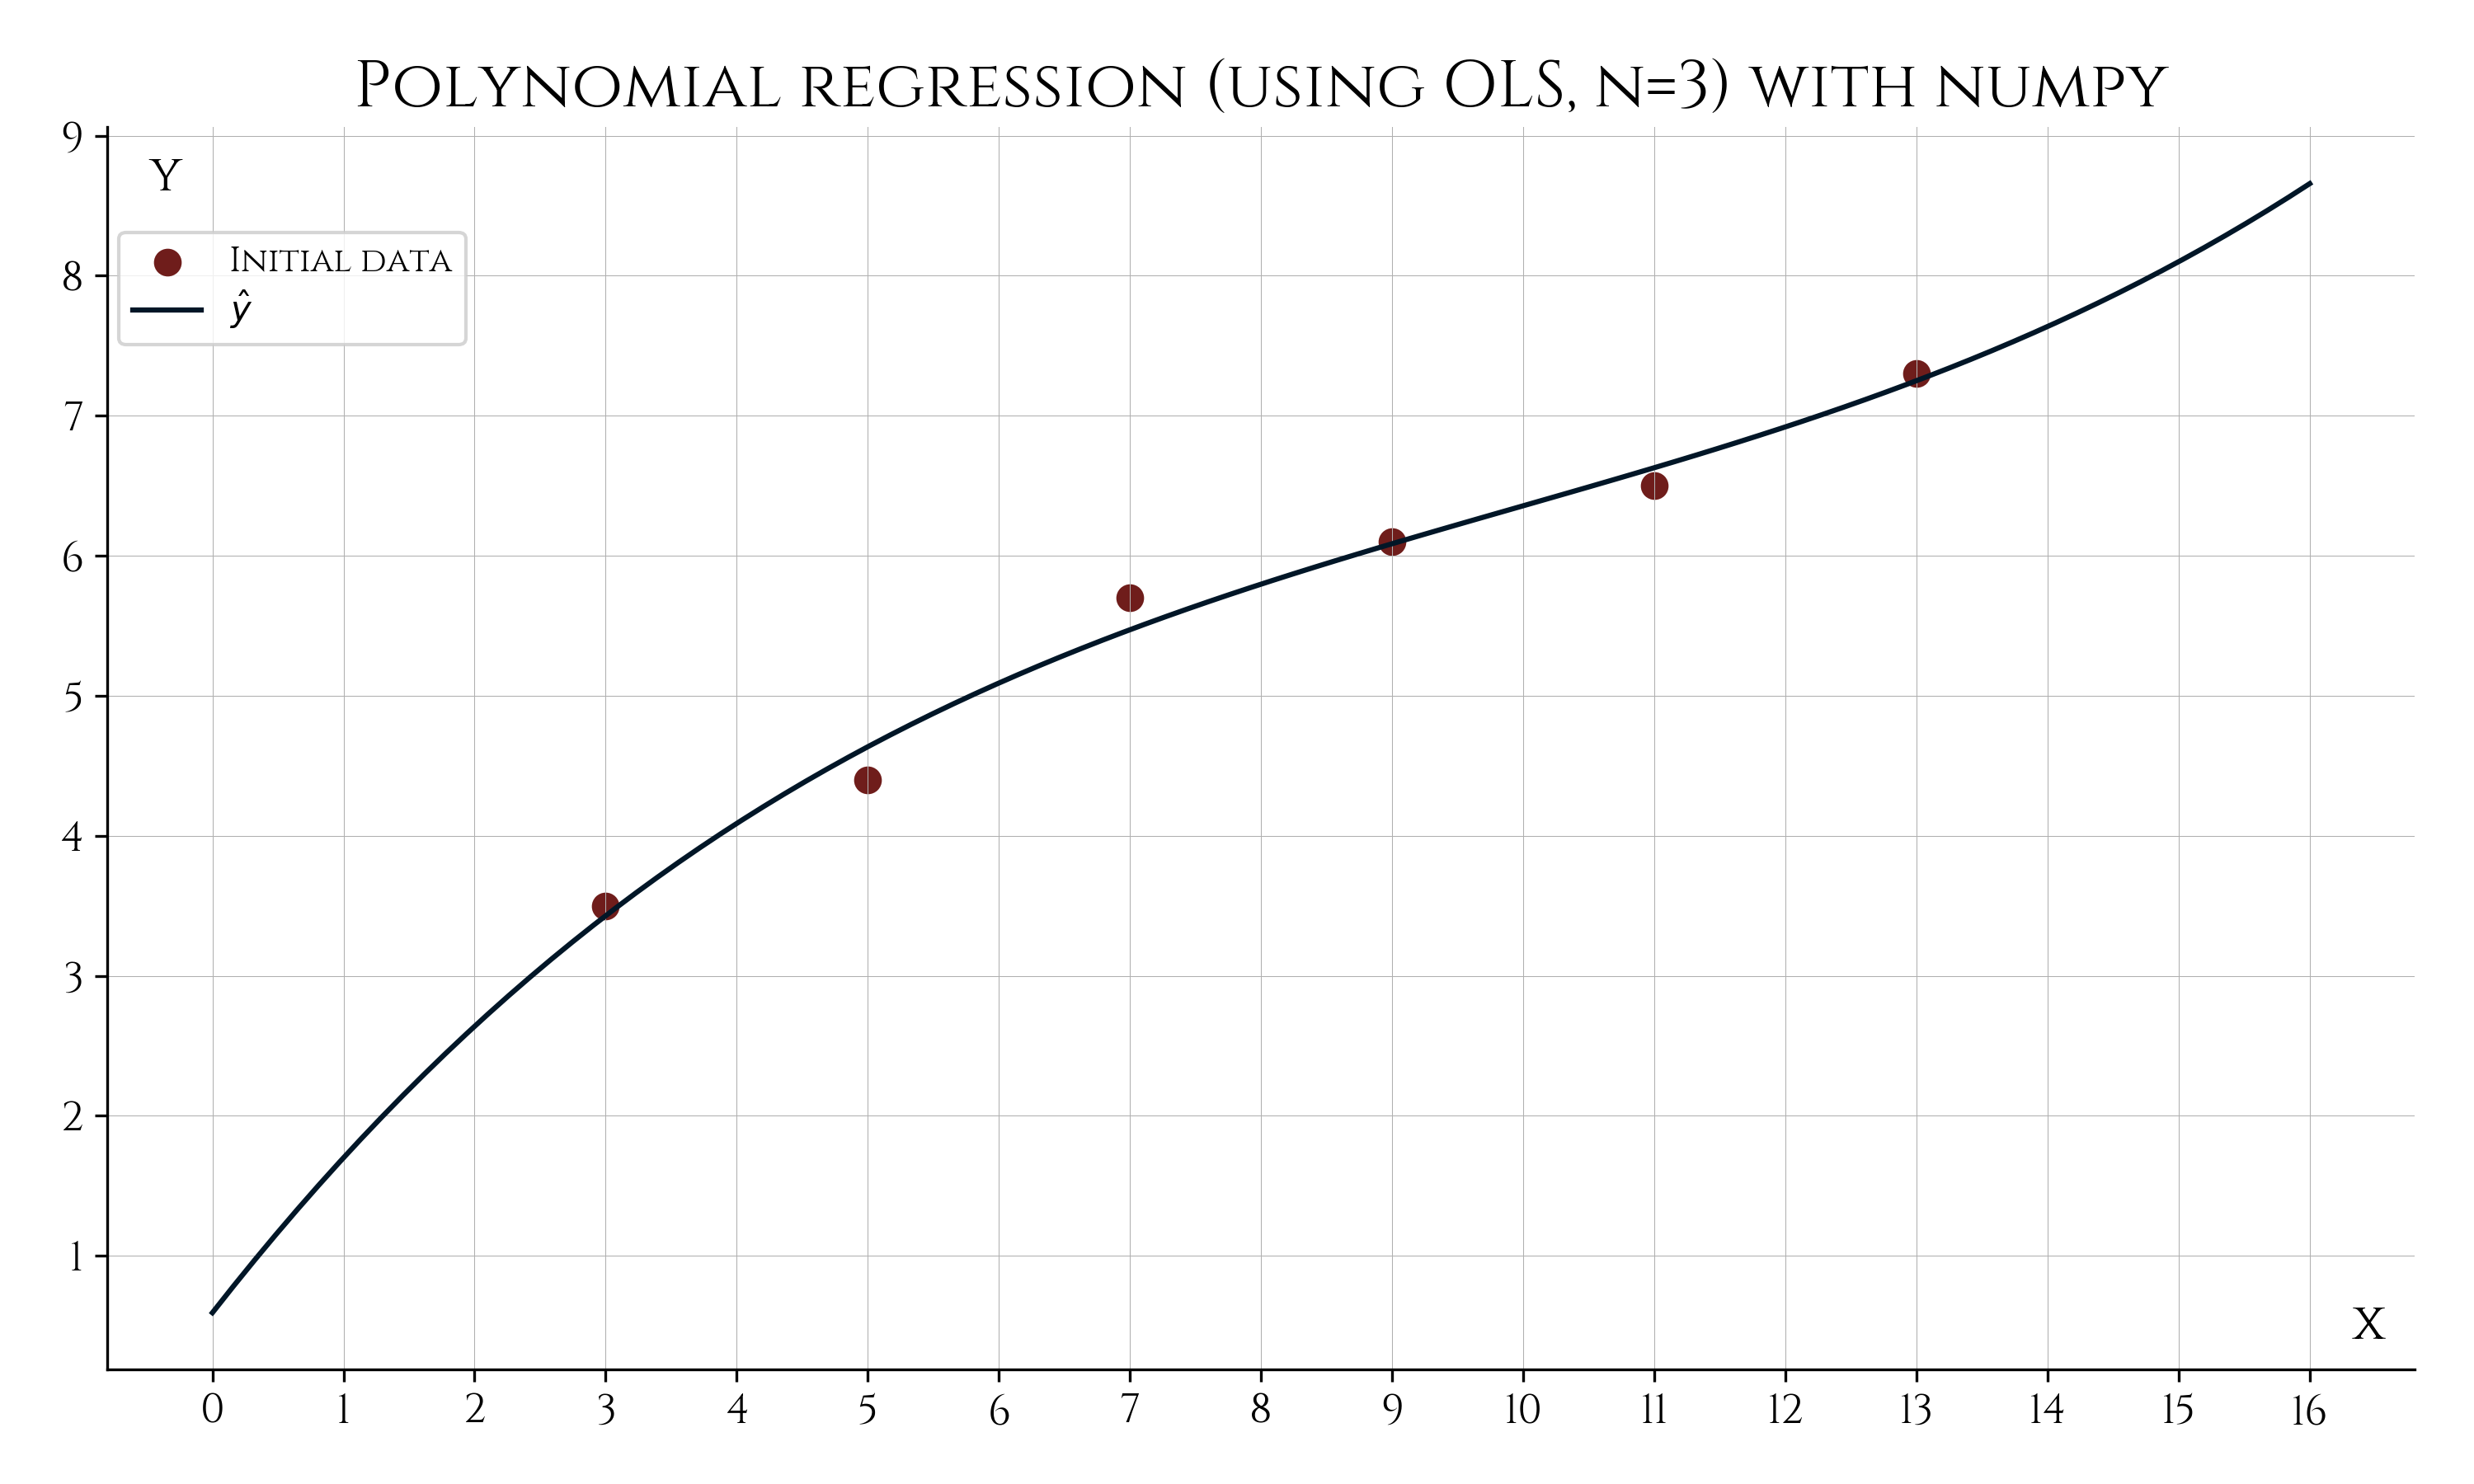
\includegraphics[width=1\textwidth, height=1\textheight, keepaspectratio]{Polynomial_Regression_numpy} \\
\end{center}

Результаты также получились аналогичными тем, что были найдены аналитически.

\subsection*{{Часть 5}}\vspace{-20pt}\rule{\linewidth}{0.1mm}
\addcontentsline{toc}{subsection}{Часть 5}

Решить задачу на языке python с использованием библиотеки scipy и matplotlib. 
Полученный результат изобразить графически при помощи библиотеки matplotlib, 
привести код для построения значений;

\subsubsection*{{Описание применяемых методов библиотеки}}\vspace{-20pt}\rule{\linewidth}{0.1mm}
\addcontentsline{toc}{subsubsection}{Описание применяемых методов библиотеки}

Воспользуемся следующими методами библиотеки \high{scipy}:

\begin{itemize}
    \item sp.linalg.inv - для нахождения обратной матрицы
\end{itemize}

\subsubsection*{{Описание хода решения}}
\addcontentsline{toc}{subsubsection}{Описание хода решения}

\paragraph*{{Линейная регрессия}}\vspace{-20pt}\rule{\linewidth}{0.1mm}
\addcontentsline{toc}{paragraph}{Линейная регрессия}

Воспользуемся матричной формой решения:

\begin{equation*}
    \beta = (X^T X)^{-1} X^T Y
\end{equation*}

Реализуем нахождение коэффициентов модели при помощи библиотеки scipy:

\begin{center}
    \begin{lstlisting}[language=Python]
X = np.array([np.ones(n_), np.array(x_values_)]).T
Y = np.array(y_values_).T
linear_scipy_beta = sp.linalg.inv((X.T @ X)) @ X.T @ Y

linear_scipy_beta
    \end{lstlisting}
\end{center}

Получим:

\begin{equation*}
    \beta_0 \approx 2.646 \qquad \beta_1 \approx 0.3671
\end{equation*}

Построим график:

\begin{center}
    \begin{lstlisting}[language=Python]
linear_scipy_func = lambda x: linear_scipy_beta[0] + linear_scipy_beta[1] * x

new_x_values = np.linspace(0, x_values_[-1] + 3, 100)
new_y_values = linear_scipy_func(new_x_values)

y_values_linear_scipy = new_y_values

buildBar('Linear_Regression_scipy', 
         '$\\hat{y}$', 
         'Linear Regression (using OLS) with scipy', 
         x_values_, 
         y_values_, 
         new_x_values, 
         new_y_values)
    \end{lstlisting}
\end{center}

\begin{center}
    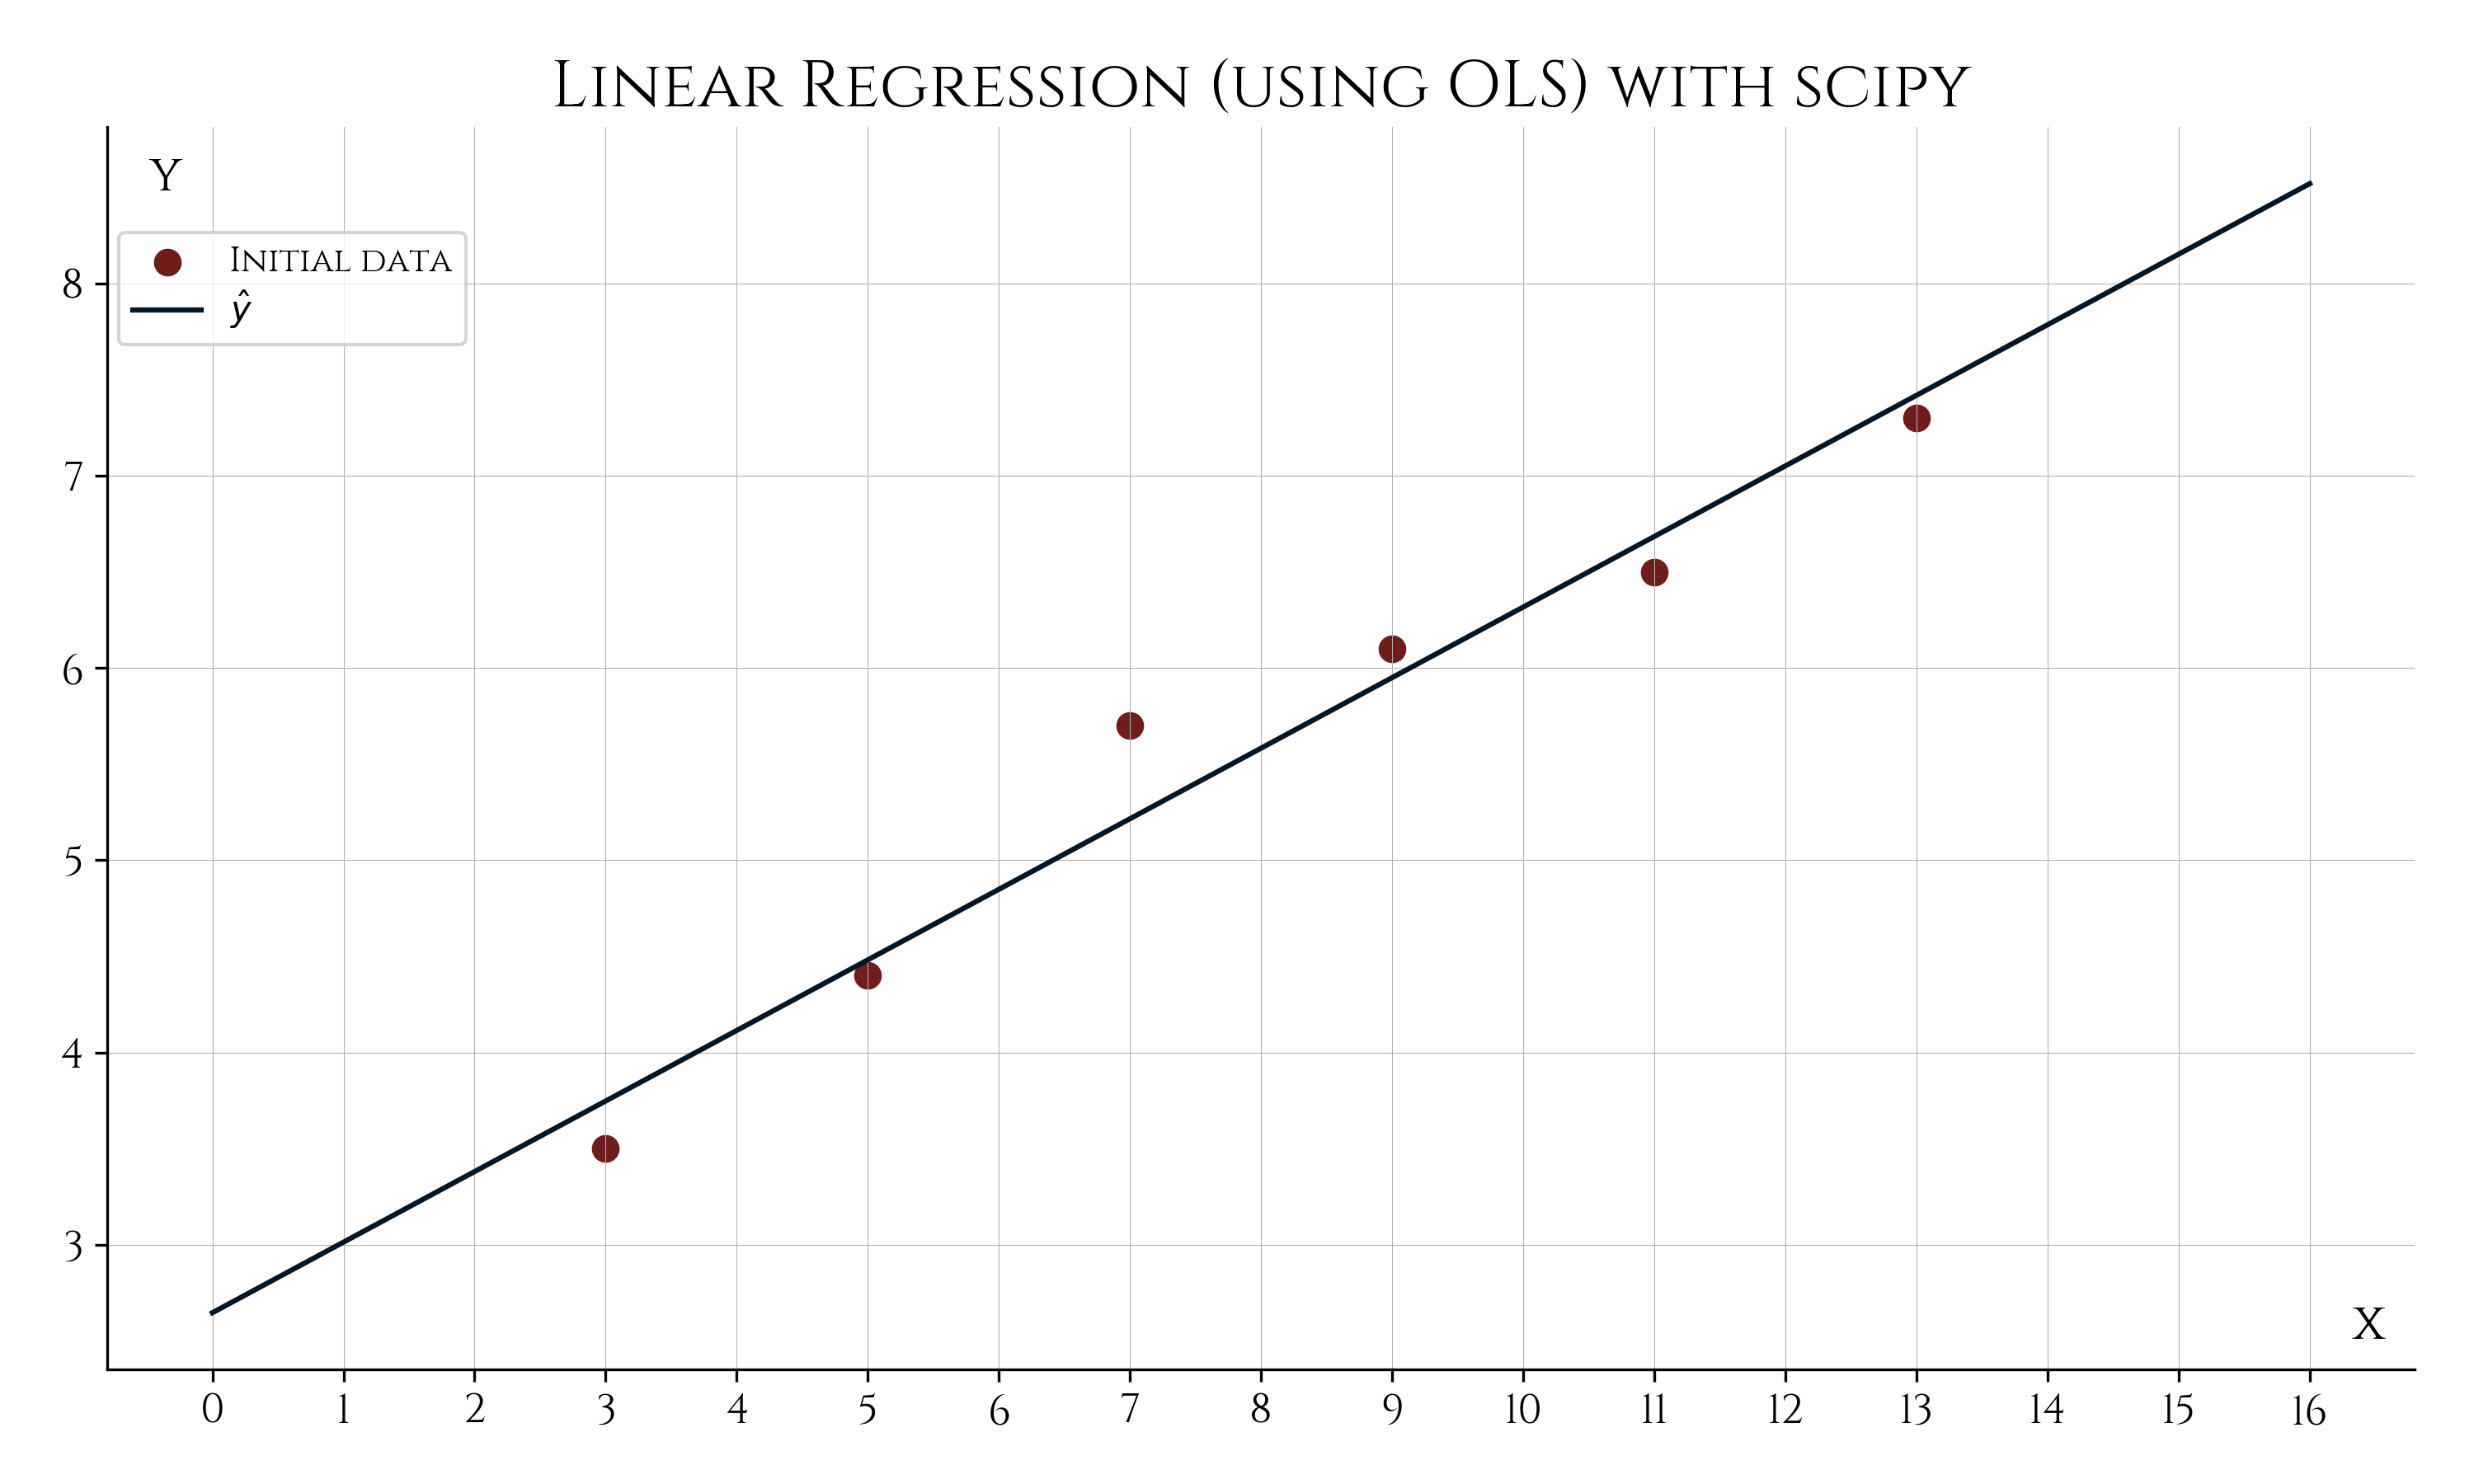
\includegraphics[width=1\textwidth, height=1\textheight, keepaspectratio]{Linear_Regression_scipy} \\
\end{center}

Результаты получились аналогичными тем, что были найдены аналитически и при помощи \high{numpy}.

\paragraph*{{Полиномиальная регрессия}}\vspace{-20pt}\rule{\linewidth}{0.1mm}
\addcontentsline{toc}{paragraph}{Полиномиальная регрессия}

Реализуем нахождение коэффициентов модели при помощи библиотеки scipy:

\begin{center}
    \begin{lstlisting}[language=Python]
X = np.array([np.ones(n_), 
              np.array(x_values_), 
              np.array(x_values_)**2, 
              np.array(x_values_)**3]).T
Y = np.array(y_values_).T
polynomial_scipy_beta = sp.linalg.inv((X.T @ X)) @ X.T @ Y

polynomial_scipy_beta
    \end{lstlisting}
\end{center}

Получим:

\begin{equation*}
    \begin{vmatrix}
        0.5933036 \\
        1.196875 \\
        -0.0933036 \\
        0.003125
    \end{vmatrix}
\end{equation*}

Построим график:

\begin{center}
    \begin{lstlisting}[language=Python]
polynomial_scipy_func = lambda x: polynomial_scipy_beta[0] + \
                                  polynomial_scipy_beta[1] * x + \
                                  polynomial_scipy_beta[2] * x**2 + \
                                  polynomial_scipy_beta[3] * x**3

new_x_values = np.linspace(0, x_values_[-1] + 3, 100)
new_y_values = polynomial_scipy_func(new_x_values)

y_values_polynomial_scipy = new_y_values

buildBar('Polynomial_Regression_scipy', 
         '$\\hat{y}$', 
         'Polynomial regression (using OLS, n=3) with scipy', 
         x_values_, 
         y_values_, 
         new_x_values, 
         new_y_values)
    \end{lstlisting}
\end{center}

\begin{center}
    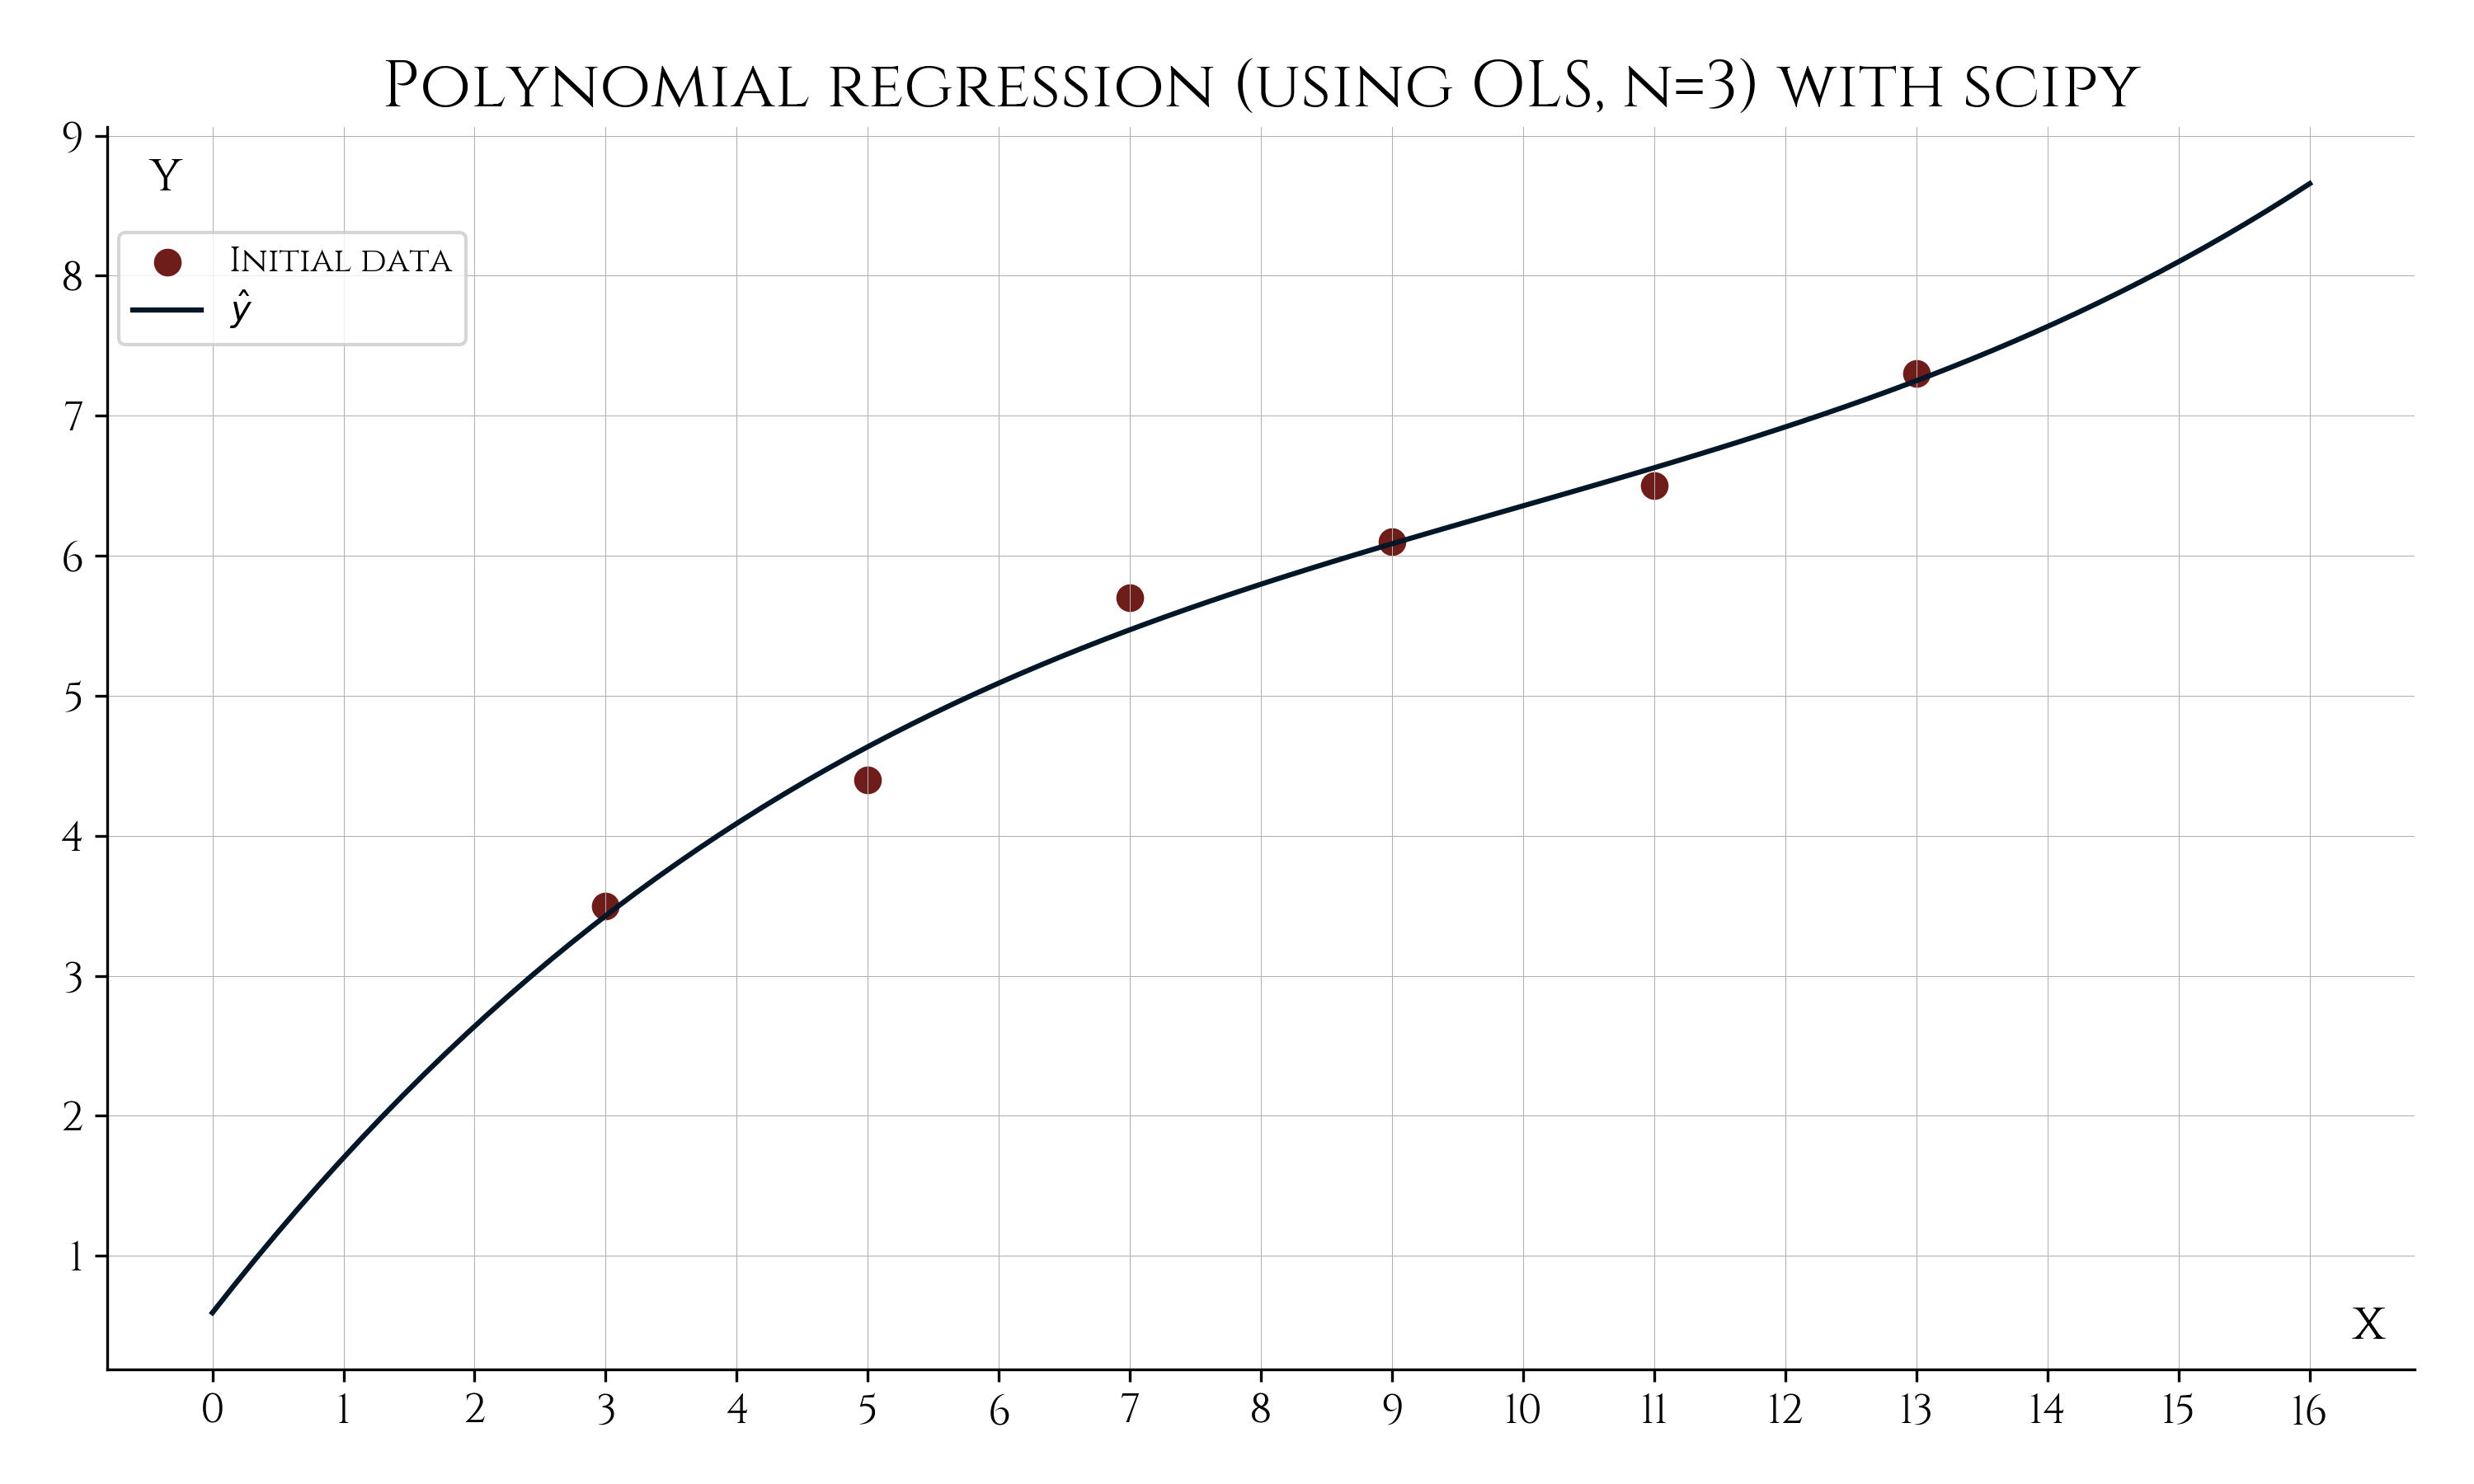
\includegraphics[width=1\textwidth, height=1\textheight, keepaspectratio]{Polynomial_Regression_scipy} \\
\end{center}

Результаты также получились аналогичными тем, что были найдены аналитически и при помощи \high{numpy}.

\subsection*{{Часть 6}}\vspace{-20pt}\rule{\linewidth}{0.1mm}
\addcontentsline{toc}{subsection}{Часть 6}

Сравнить решения, полученные вручную и с помощью решения на python, построить решения графически.  
Оценить точность полученных решений.

\subsubsection*{{Построение совмещенных графиков}}\vspace{-20pt}\rule{\linewidth}{0.1mm}
\addcontentsline{toc}{subsubsection}{Построение совмещенных графиков}

Графики изобразим с разной толщиной, чтобы было видно как они накладываются друг на друга.

\paragraph*{{Линейная регрессия}}\vspace{-20pt}\rule{\linewidth}{0.1mm}
\addcontentsline{toc}{paragraph}{Линейная регрессия}

Построим графики:

\begin{center}
    \begin{lstlisting}[language=Python]
def buildBar(filename):
    _, ax = plt.subplots(figsize=(10, 6))

    ax.scatter(x_values_, 
               y_values_, 
               color=RED,
               s=50,
               label='Initial data',
               zorder=5)

    universal_x_values = np.linspace(0, x_values_[-1] + 3, 100)

    ax.plot(universal_x_values, 
            y_values_hand_approximation, 
            linestyle=':', l
            inewidth=2, 
            color='black', 
            label='Hand Approximation', 
            zorder=4)
    ax.plot(universal_x_values, 
            y_values_linear_analytical, 
            linewidth=10, 
            label='Analytical Linear Regression', 
            zorder=1)
    ax.plot(universal_x_values, 
            y_values_linear_numpy, 
            linewidth=5, 
            label='Linear Regression (numpy)', 
            zorder=2)
    ax.plot(universal_x_values, 
            y_values_linear_scipy, 
            linewidth=1, 
            label='Linear Regression (scipy)', 
            zorder=3)

    plt.grid(linestyle='-', linewidth=0.25)

    ax.set_title('Combined Linear plots')
    decorate_plot(ax, np.arange(universal_x_values[0], 
                                universal_x_values[-1]+1, 1), 
                                'x', 
                                'y', 
                                loc=(0.005, 0.725))
    
    if SAVE_PLOTS:
        plt.savefig(f'images/{filename}.png', dpi=300, transparent=True)

    plt.show()

buildBar('Combined_Linear_Plots')
    \end{lstlisting}
\end{center}

\begin{center}
    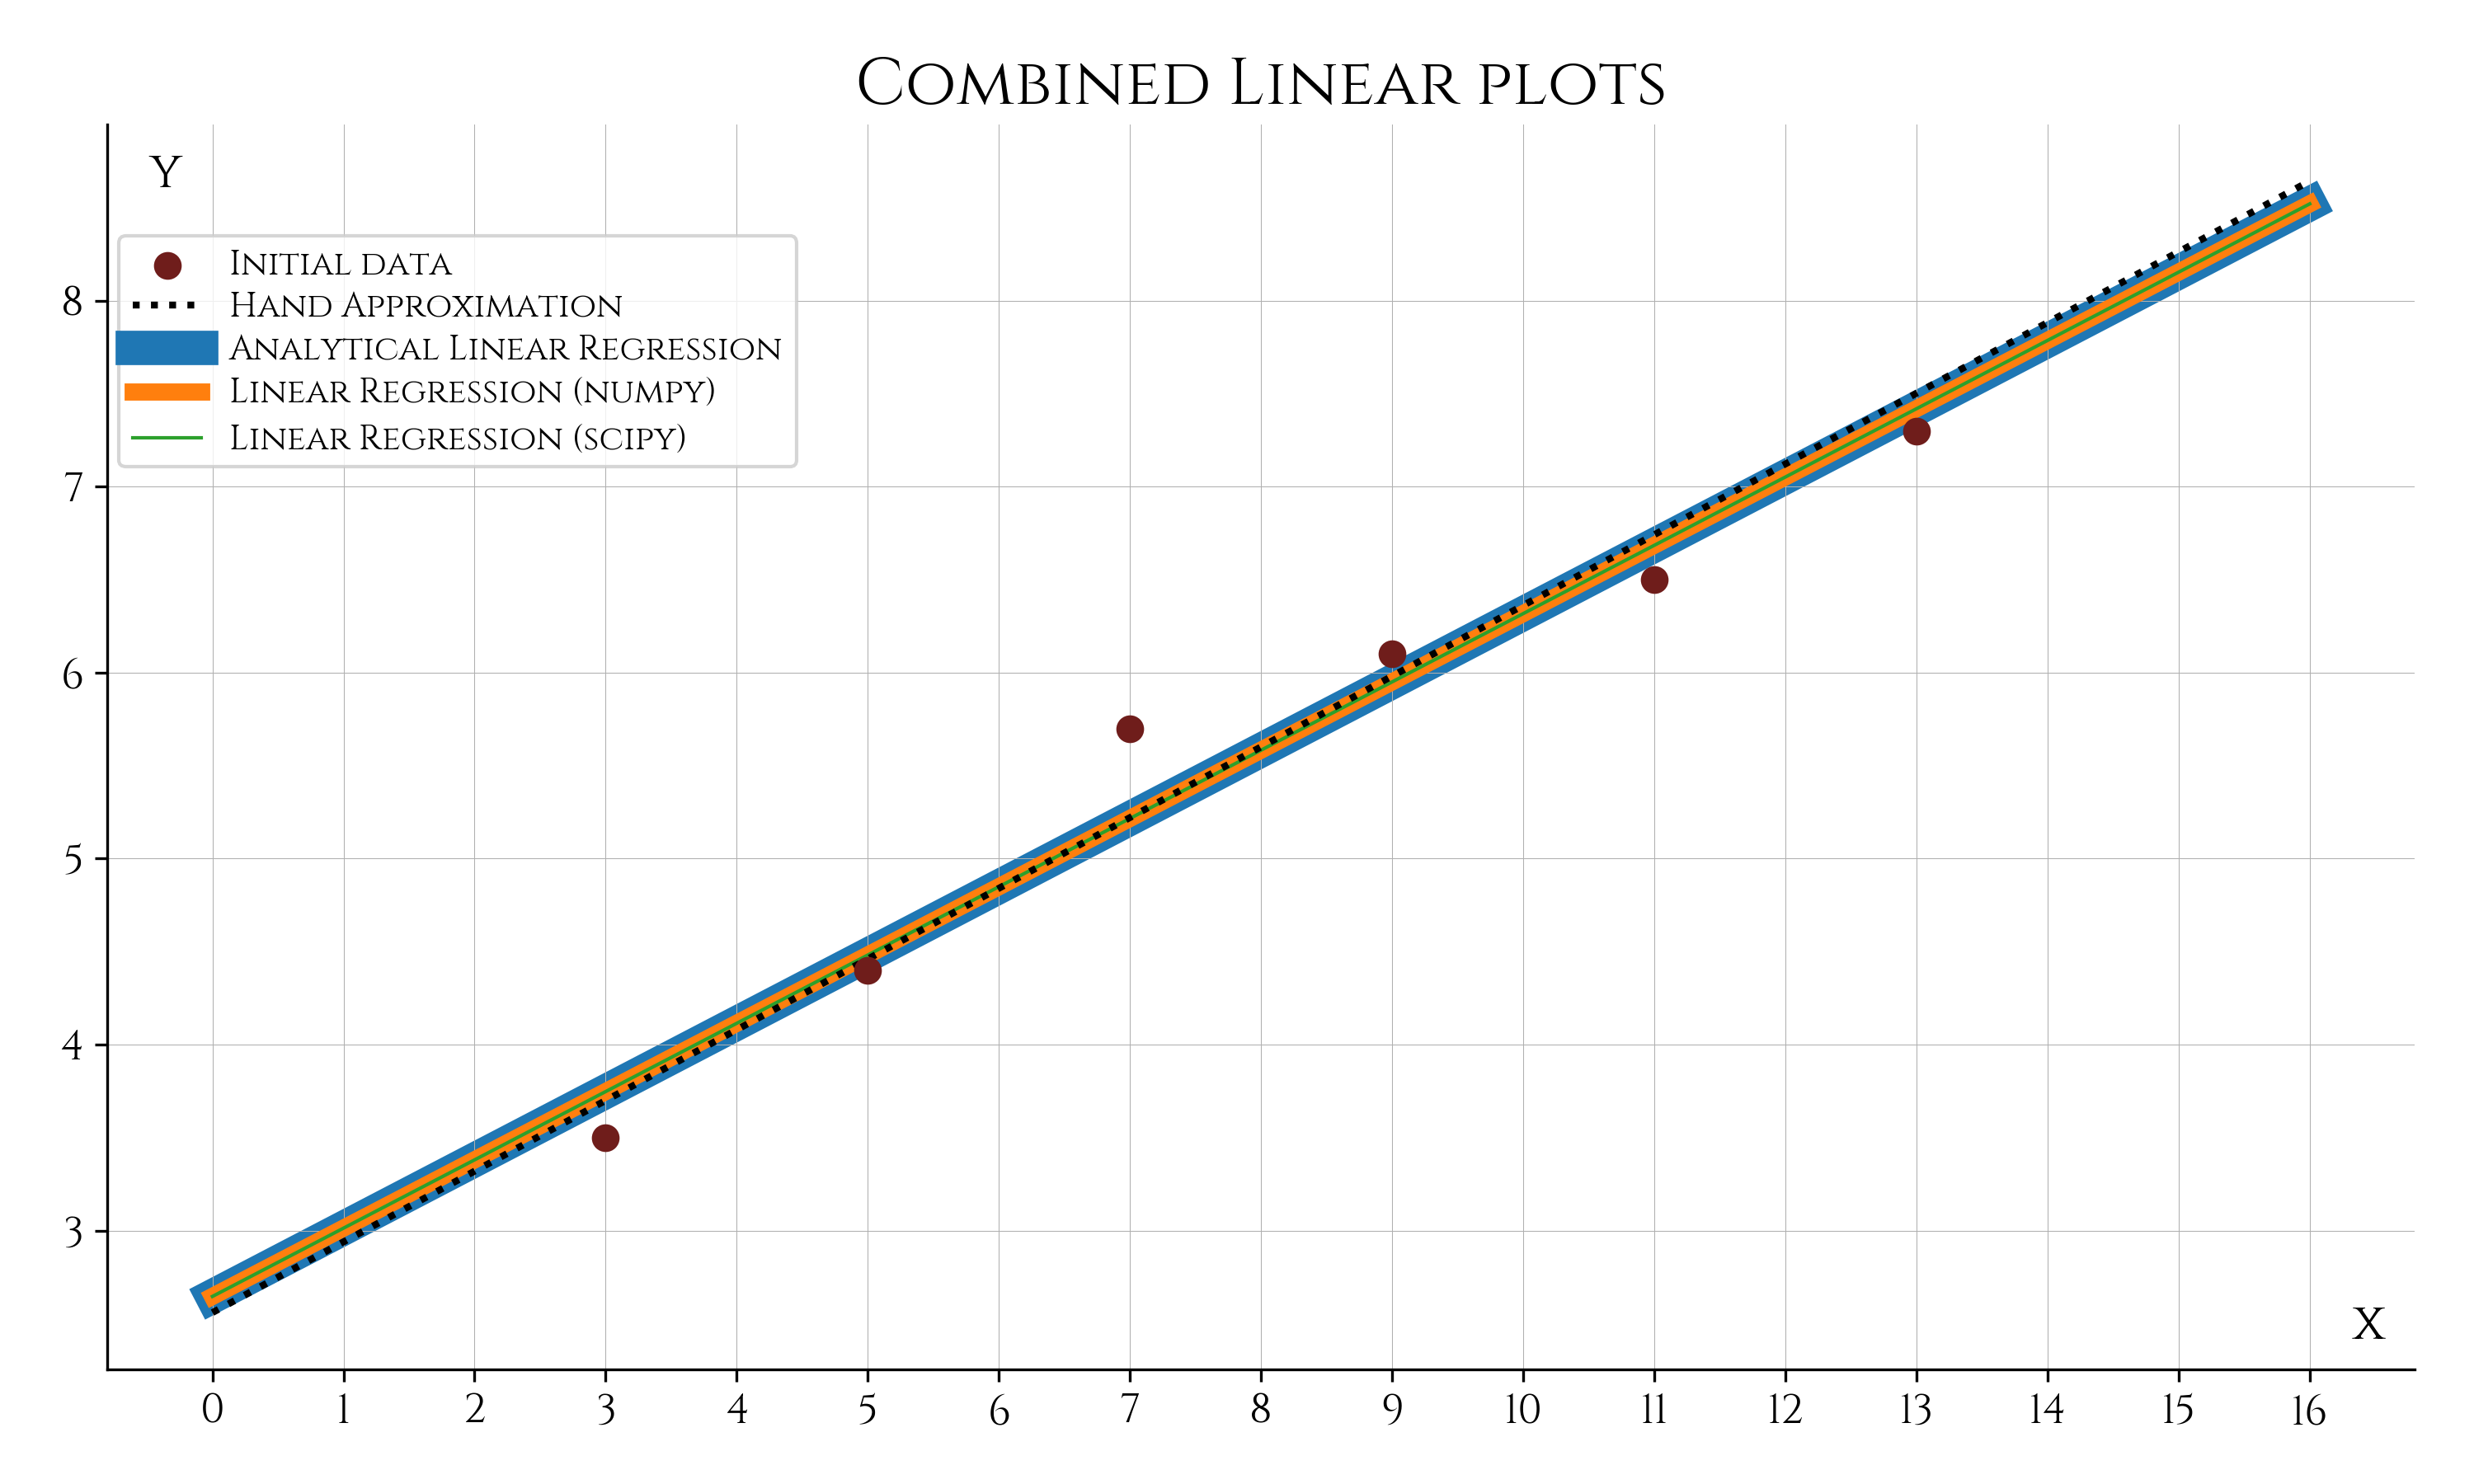
\includegraphics[width=1\textwidth, height=1\textheight, keepaspectratio]{Combined_Linear_Plots} \\
\end{center}

Графики, построенные по моделям, чьи коэффициенты были найдены аналитически, при помощи numpy и scipy 
идеально наложились друг на друга. График, построенный вручную слегка смещен.

\paragraph*{{Полиномиальная регрессия}}\vspace{-20pt}\rule{\linewidth}{0.1mm}
\addcontentsline{toc}{paragraph}{Полиномиальная регрессия}

Построим графики:

\begin{center}
    \begin{lstlisting}[language=Python]
def buildBar(filename):
    _, ax = plt.subplots(figsize=(10, 6))

    ax.scatter(x_values_, 
               y_values_, 
               color=RED,
               s=50,
               label='Initial data', 
               zorder=4)

    universal_x_values = np.linspace(0, x_values_[-1] + 3, 100)

    ax.plot(universal_x_values, 
            y_values_polynomial_analytical, 
            linewidth=10, 
            label='Analytical Polynomial Regression', 
            zorder=1)
    ax.plot(universal_x_values, 
            y_values_polynomial_numpy, 
            linewidth=5, 
            label='Polynomial Regression (numpy)', 
            zorder=2)
    ax.plot(universal_x_values, 
            y_values_polynomial_scipy, 
            linewidth=1, 
            label='Polynomial Regression (scipy)', 
            zorder=3)

    plt.grid(linestyle='-', linewidth=0.25)

    ax.set_title('Combined Polynomial plots')
    decorate_plot(ax, np.arange(universal_x_values[0], 
                                universal_x_values[-1]+1, 1), 'x', 'y', loc=(0.005, 
                                                                             0.75))
    
    if SAVE_PLOTS:
        plt.savefig(f'images/{filename}.png', dpi=300, transparent=True)

    plt.show()

buildBar('Combined_Polynomial_Plots')
    \end{lstlisting}
\end{center}

\begin{center}
    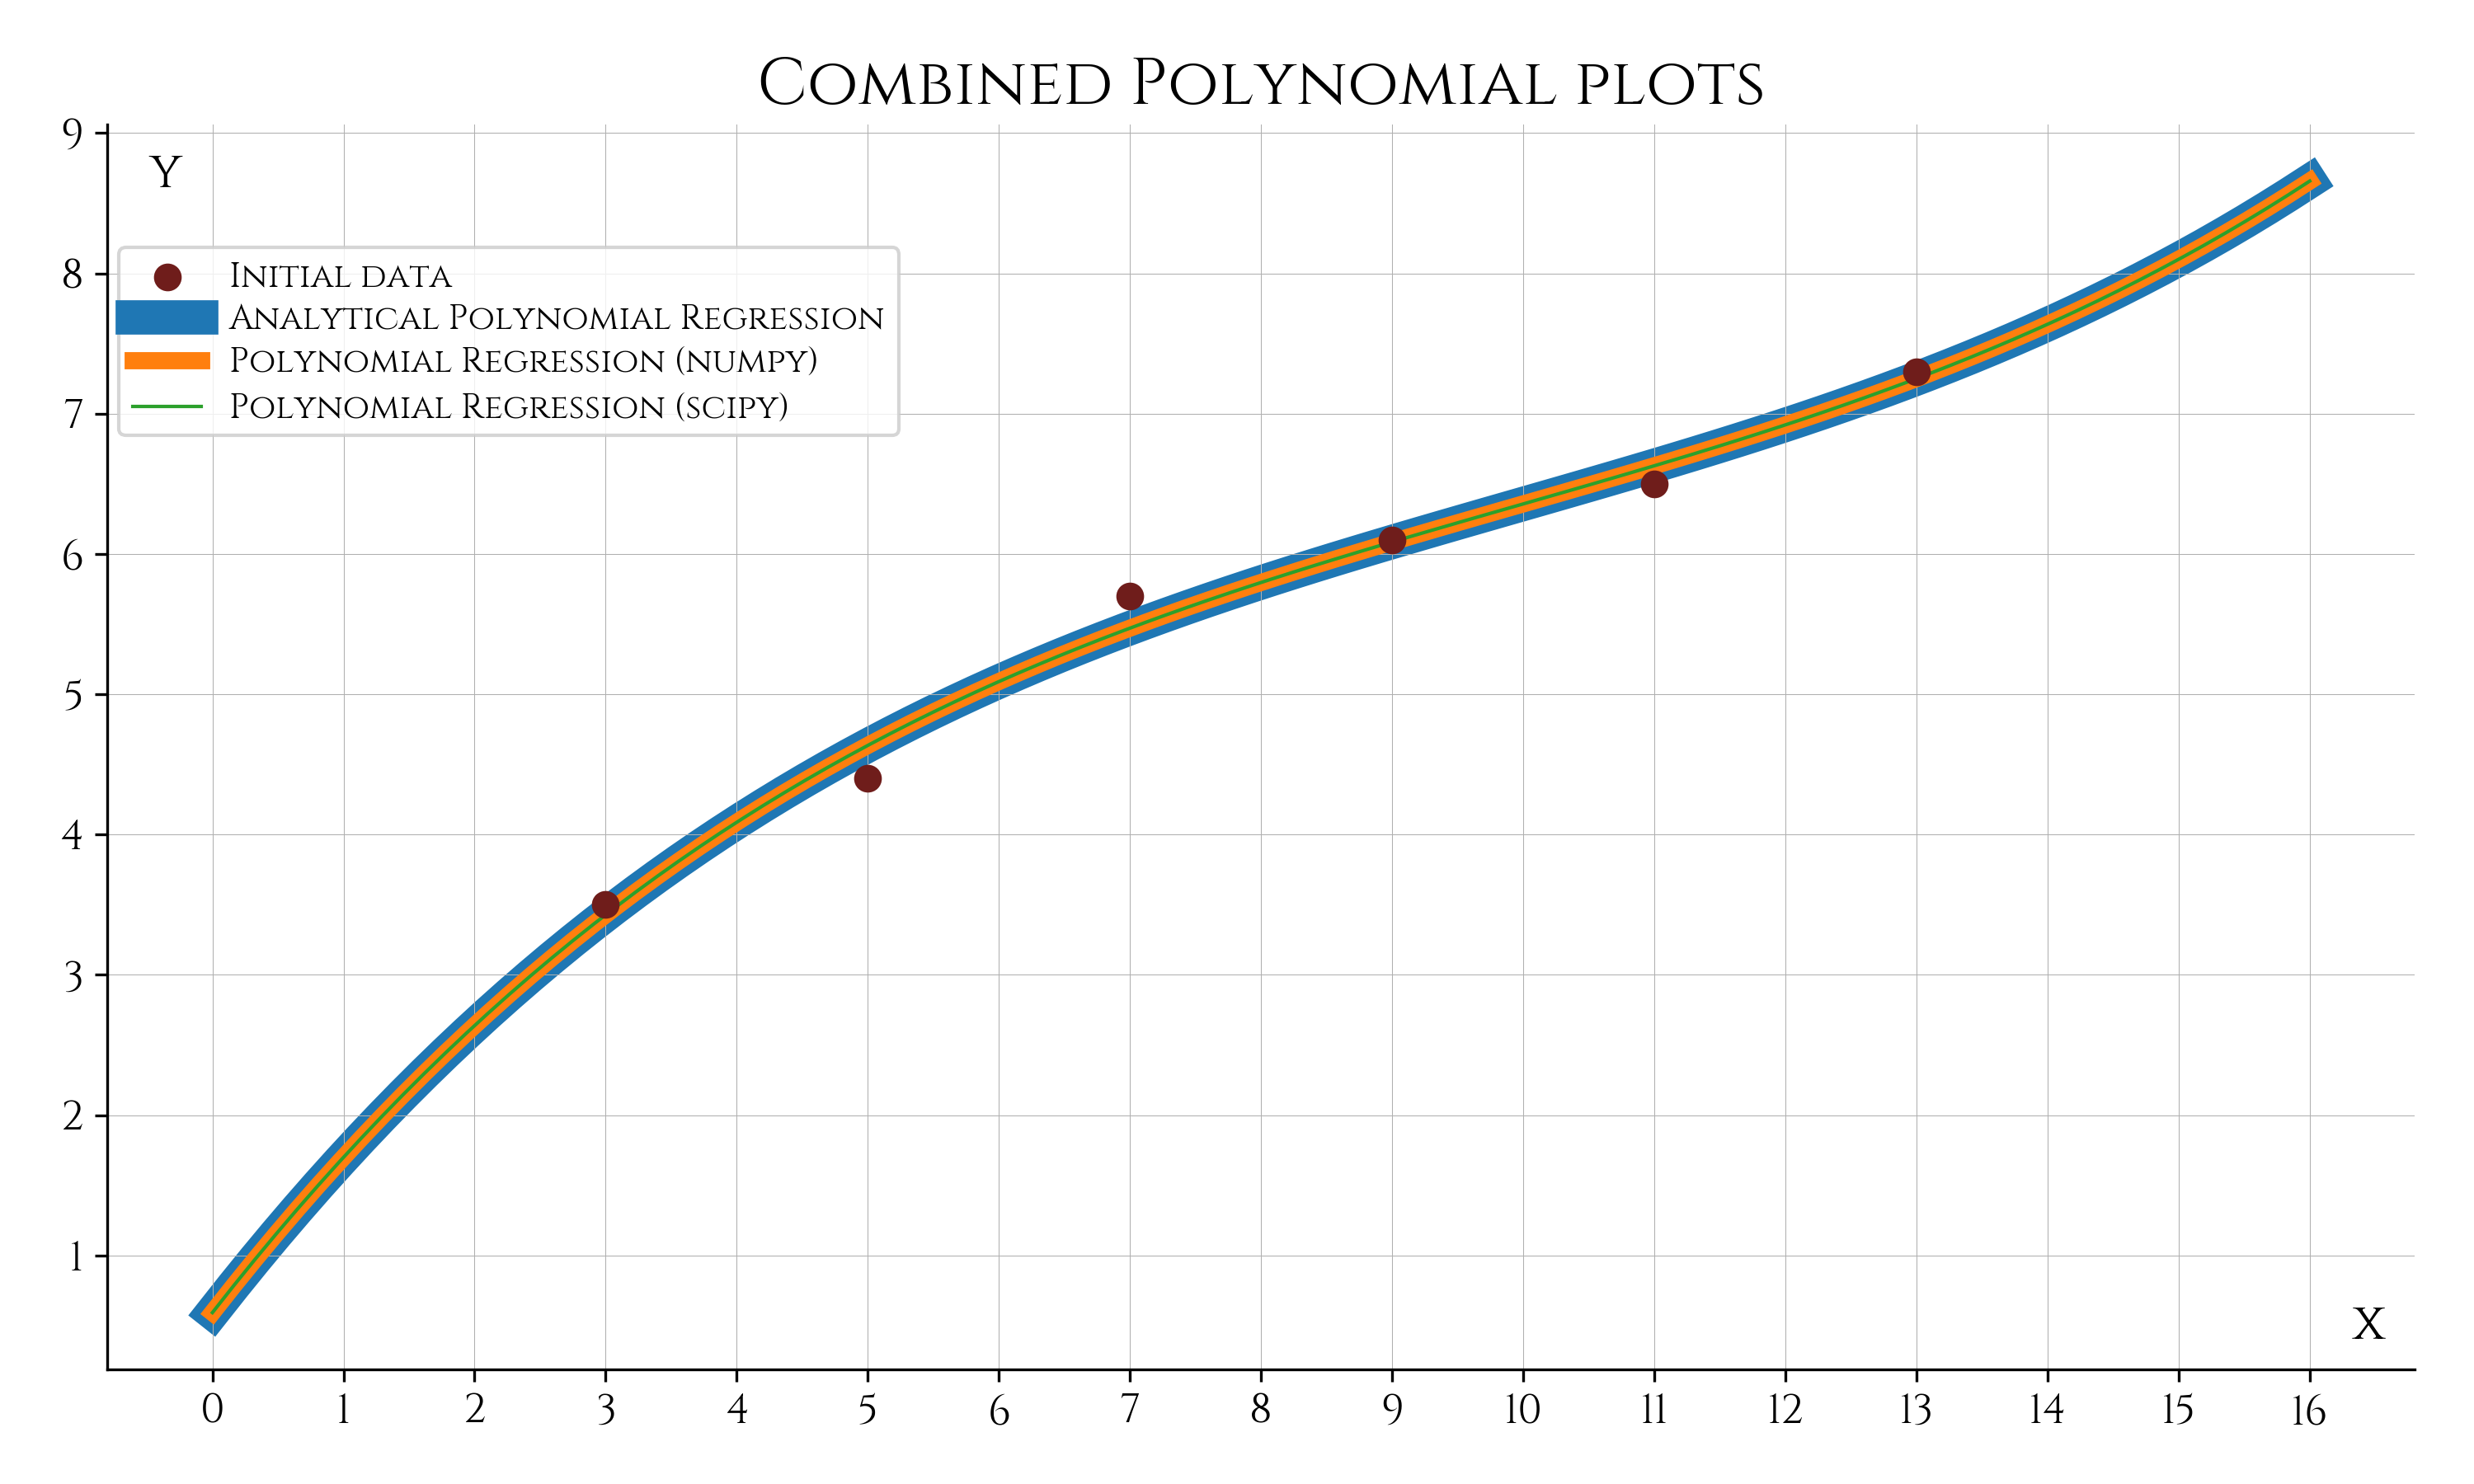
\includegraphics[width=1\textwidth, height=1\textheight, keepaspectratio]{Combined_Polynomial_Plots} \\
\end{center}

Графики, построенные по моделям, чьи коэффициенты были найдены аналитически, при помощи numpy и scipy 
идеально наложились друг на друга.

\subsubsection*{{Сравнение коэффициентов}}\vspace{-20pt}\rule{\linewidth}{0.1mm}
\addcontentsline{toc}{subsubsection}{Сравнение коэффициентов}

Вычтем коэффициенты для линейных и полиномиальных моделей, полученные разными способами 
друг из друга и найдём среднее значение векторов:

\begin{center}
    \begin{lstlisting}[language=Python]
print(np.mean(y_values_hand_approximation-y_values_linear_analytical))
print(np.mean(y_values_hand_approximation-y_values_linear_numpy))
print(np.mean(y_values_hand_approximation-y_values_linear_scipy))

print('-'*200)

print(np.mean(y_values_linear_analytical-y_values_linear_numpy))
print(np.mean(y_values_linear_numpy-y_values_linear_scipy))
print(np.mean(y_values_linear_scipy-y_values_linear_analytical))

print('-'*200)

print(np.mean(y_values_polynomial_analytical-y_values_polynomial_numpy))
print(np.mean(y_values_polynomial_numpy-y_values_polynomial_scipy))
print(np.mean(y_values_polynomial_scipy-y_values_polynomial_analytical))
    \end{lstlisting}
\end{center}

Получим:

\begin{gather*}
    0.017807351077313804\\
    0.017807351077314702\\
    0.017807351077314702\\[2em]
    9.01501095995627e-16\\
    0.0\\
    -9.01501095995627e-16\\[2em]
    1.29910158852553e-9\\
    -9.558054347991174e-12\\
    -1.28954353417754e-9\\
\end{gather*}

Что говорит о том, что погрешность вычисления коэффициентов разными способами пренебрежительно мала.

\newpage

\subsection*{{Часть 7}}\vspace{-20pt}\rule{\linewidth}{0.1mm}
\addcontentsline{toc}{subsection}{Часть 7}

С помощью полученной модели предсказать значения y для значений x = 4,5; x = 5.

\subsubsection*{{Предсказание}}\vspace{-20pt}\rule{\linewidth}{0.1mm}
\addcontentsline{toc}{subsubsection}{Предсказание}

Подставим x = 4,5; x = 5 в каждую из моделей:

\begin{center}
    \begin{lstlisting}[language=Python]
@dataclass
class Func:
    name: str
    func: Callable

funcs = [
    Func('Hand approximation',               hand_func),
    Func('Linear Analytical Regression',     linear_analytical_func),
    Func('Polynomial Analytical Regression', polynomial_analytical_func),
    Func('Linear Regression (numpy)',        linear_numpy_func),
    Func('Polynomial Regression (numpy)',    polynomial_numpy_func),
    Func('Linear Regression (scipy)',        linear_scipy_func),
    Func('Polynomial Regression (scipy)',    polynomial_scipy_func)
]

x_data = [4.5, 5]

for func in funcs:
    for x in x_data:
        print(f'Calculating x = {x} with {func.name}, result: {func.func(x)}')
    \end{lstlisting}
\end{center}

Итого:

\begin{table}[h!]
    \centering
    \renewcommand{\arraystretch}{1.5} % Increase the vertical space between rows
    \begin{tabular}{lcc}
    \toprule
    \textbf{Method} & \textbf{Result for \( x = 4.5 \)} & \textbf{Result for \( x = 5 \)} \\
    \midrule
    Hand approximation & 4.270342205323194 & 4.460456273764259 \\
    Linear Analytical Regression & 4.298333333333333 & 4.481904761904762 \\
    Polynomial Analytical Regression & 4.37460937545060 & 4.63571428619517 \\
    Linear Regression (numpy) & 4.298333333333332 & 4.481904761904761 \\
    Polynomial Regression (numpy) & 4.374609374991685 & 4.635714285706156 \\
    Linear Regression (scipy) & 4.298333333333332 & 4.481904761904761 \\
    Polynomial Regression (scipy) & 4.374609375000244 & 4.6357142857146165 \\
    \bottomrule
    \end{tabular}
\end{table}

Изобразим результаты графически (так как все точки либо накладываются, 
либо находятся близко друг к другу, зададим для каждой из точек разный размер):

\begin{center}
    \begin{lstlisting}[language=Python]
def buildBar(filename):
    _, ax = plt.subplots(figsize=(10, 6))

    # initial data
    ax.scatter(x_values_, 
               y_values_, 
               color=RED,
               s=50,
               label='Initial data', 
               zorder=2)

    # analytical polynomial regression
    universal_x_values = np.linspace(0, x_values_[-1] + 3, 100)

    ax.plot(universal_x_values, 
            y_values_polynomial_analytical,
            linewidth=2, 
            label='Analytical Polynomial Regression', 
            zorder=1, 
            color=RICH_BLACK)

    # predicted values
    methods = [
        "Hand approximation",
        "Analytical Linear Regression",
        "Analytical Polynomial Regression",
        "Linear Regression (numpy)",
        "Polynomial Regression (numpy)",
        "Linear Regression (scipy)",
        "Polynomial Regression (scipy)",
    ]

    x_values = [4.5, 5]
    results = {
        "Hand approximation": [4.270342205323194, 4.460456273764259],
        "Analytical Linear Regression": [4.298333333333333, 4.481904761904762],
        "Analytical Polynomial Regression": [4.37460937545060, 4.63571428619517],
        "Linear Regression (numpy)": [4.298333333333332, 4.481904761904761],
        "Polynomial Regression (numpy)": [4.374609374991685, 4.635714285706156],
        "Linear Regression (scipy)": [4.298333333333332, 4.481904761904761],
        "Polynomial Regression (scipy)": [4.374609375000244, 4.6357142857146165],
    }

    i = 3
    for method in methods:
        plt.scatter(x_values, 
                    results[method], 
                    label=method, 
                    s=50 + 100 * (i-2), 
                    zorder=12-i)
        print(50 + 25 * (i-2), 12-i)
        i += 1

    plt.grid(linestyle='-', linewidth=0.25)

    ax.set_title('Prediction')
    decorate_plot(ax, np.arange(universal_x_values[0], 
                                universal_x_values[-1]+1, 1), 
                                'x', 
                                'y', 
                                loc=(0.005, 0.6))
    
    if SAVE_PLOTS:
        plt.savefig(f'images/{filename}.png', dpi=300, transparent=True)

    plt.show()

buildBar('Prediction_Plot')
    \end{lstlisting}
\end{center}

\begin{center}
    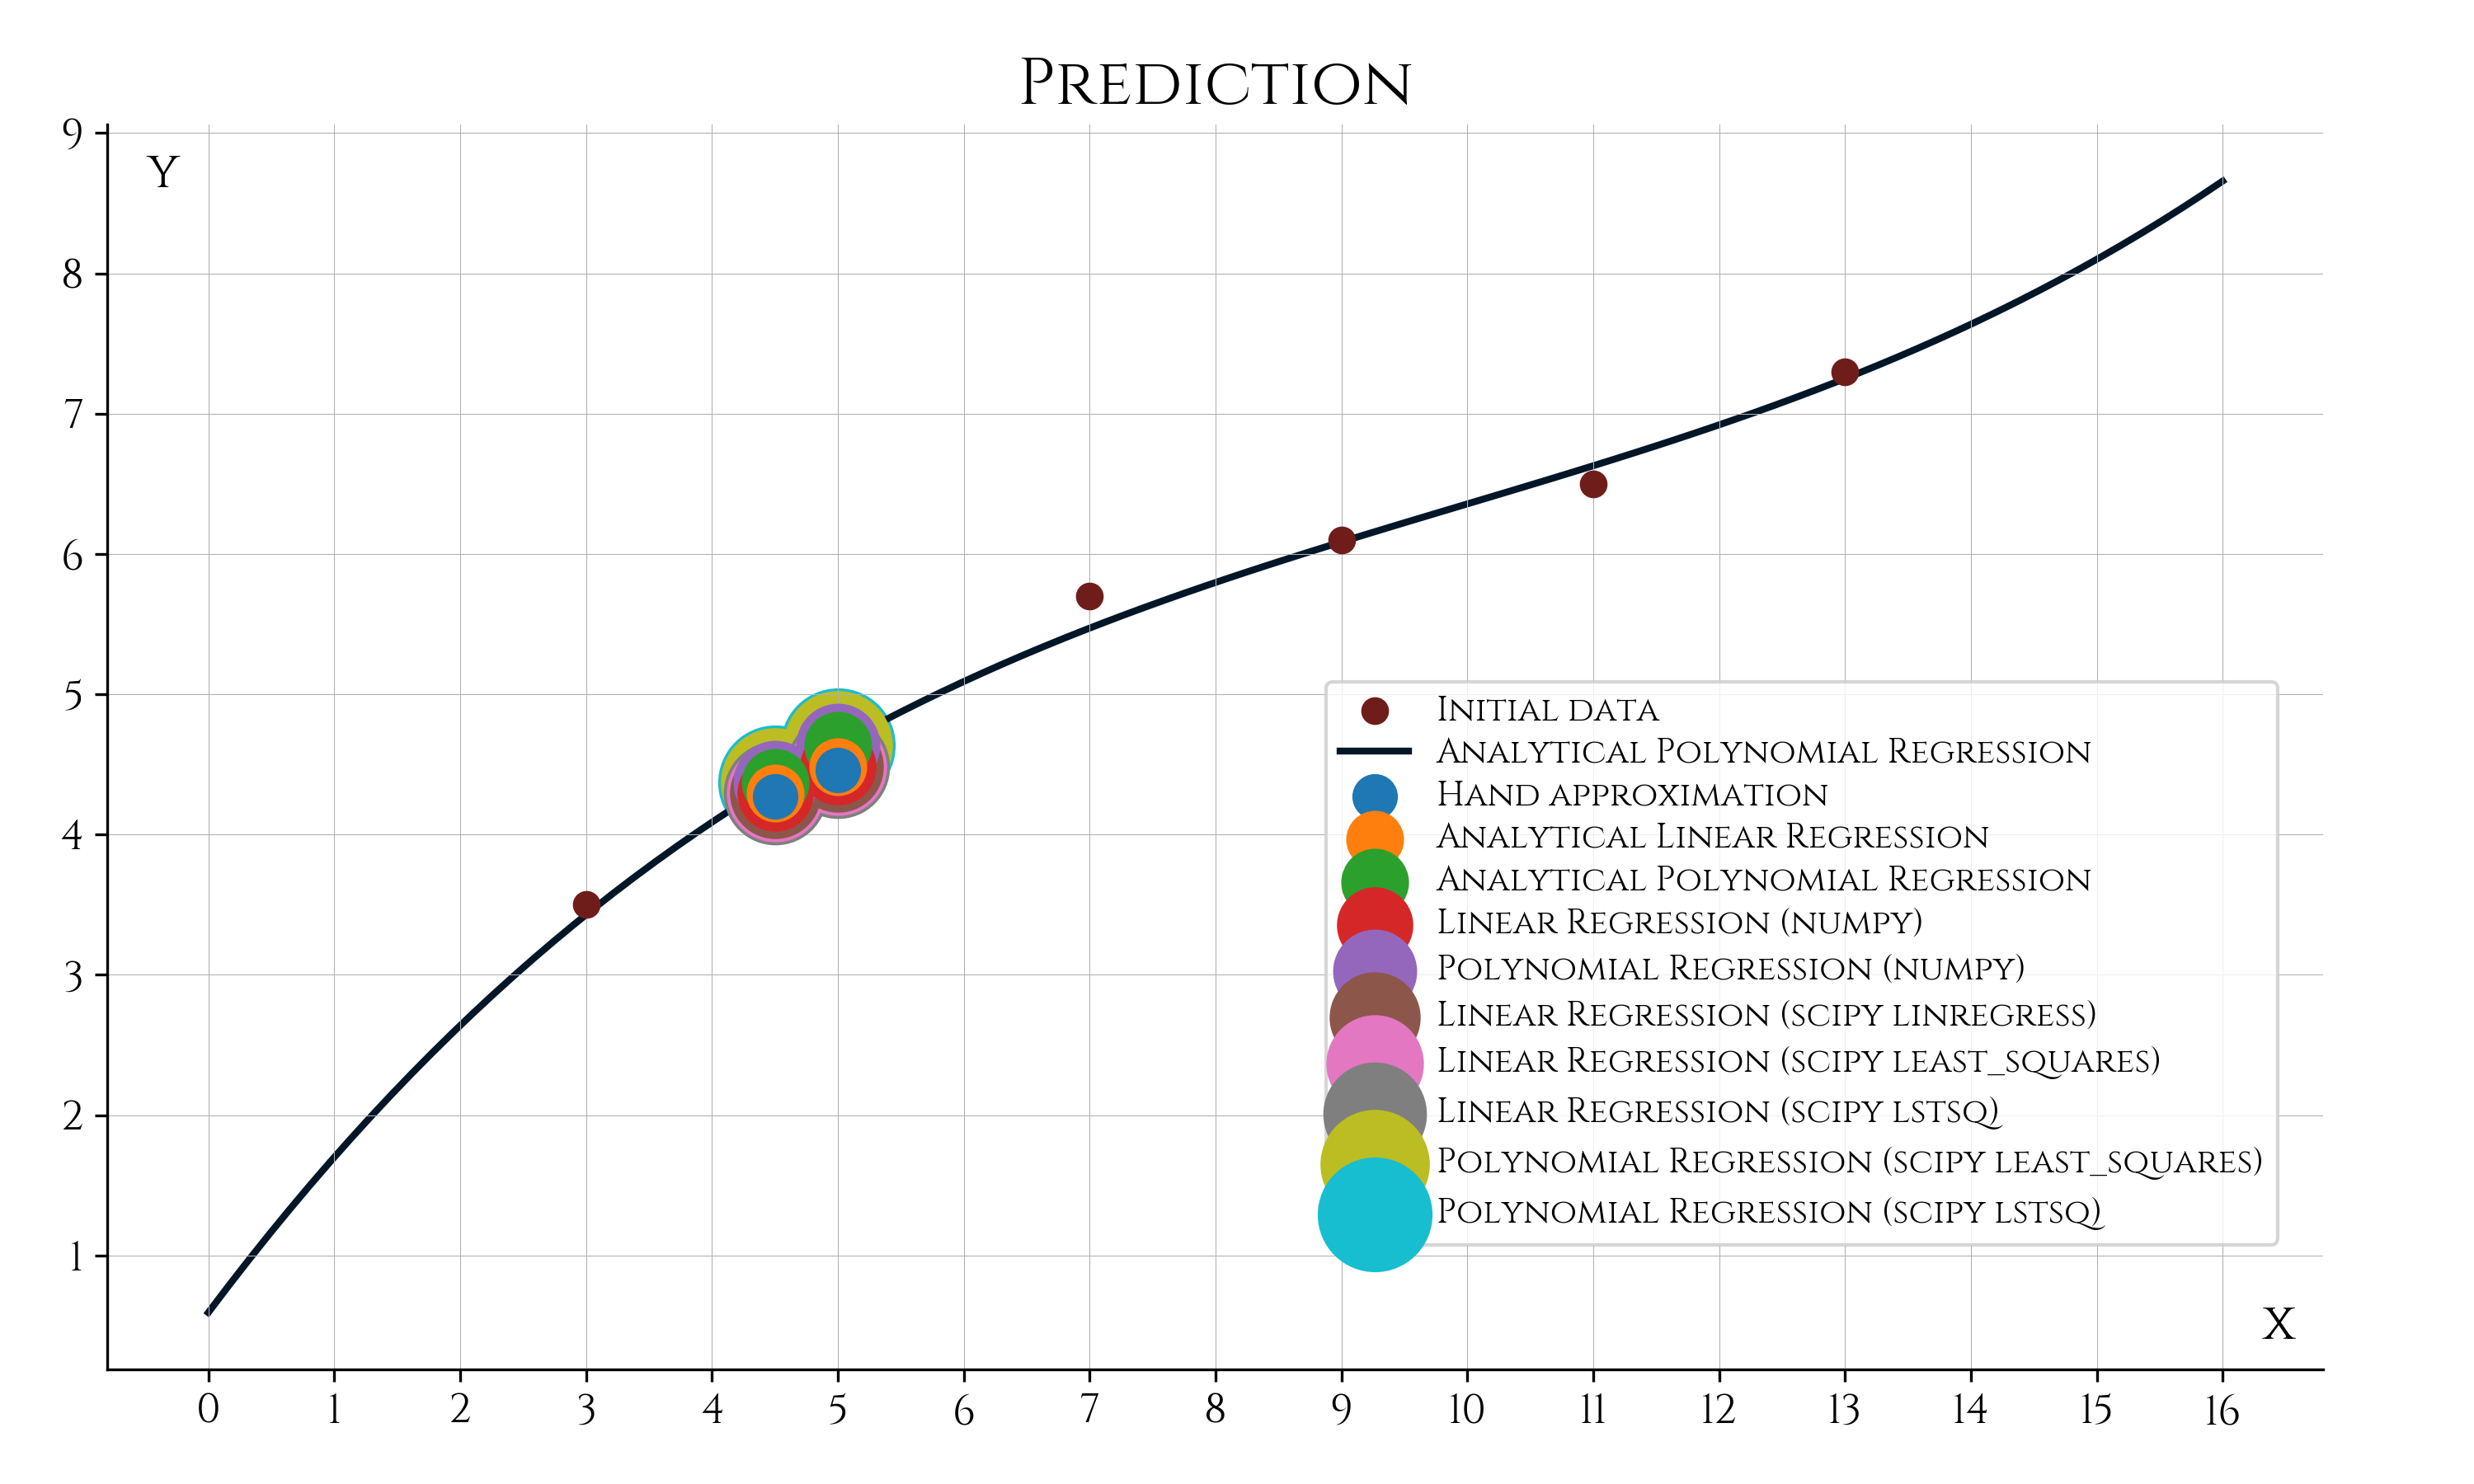
\includegraphics[width=1\textwidth, height=1\textheight, keepaspectratio]{Prediction_Plot} \\
\end{center}

\end{document}
